% Options for packages loaded elsewhere
\PassOptionsToPackage{unicode}{hyperref}
\PassOptionsToPackage{hyphens}{url}
%
\documentclass[
  ignorenonframetext,
]{beamer}
\usepackage{pgfpages}
\setbeamertemplate{caption}[numbered]
\setbeamertemplate{caption label separator}{: }
\setbeamercolor{caption name}{fg=normal text.fg}
\beamertemplatenavigationsymbolsempty
% Prevent slide breaks in the middle of a paragraph
\widowpenalties 1 10000
\raggedbottom
\setbeamertemplate{part page}{
  \centering
  \begin{beamercolorbox}[sep=16pt,center]{part title}
    \usebeamerfont{part title}\insertpart\par
  \end{beamercolorbox}
}
\setbeamertemplate{section page}{
  \centering
  \begin{beamercolorbox}[sep=12pt,center]{part title}
    \usebeamerfont{section title}\insertsection\par
  \end{beamercolorbox}
}
\setbeamertemplate{subsection page}{
  \centering
  \begin{beamercolorbox}[sep=8pt,center]{part title}
    \usebeamerfont{subsection title}\insertsubsection\par
  \end{beamercolorbox}
}
\AtBeginPart{
  \frame{\partpage}
}
\AtBeginSection{
  \ifbibliography
  \else
    \frame{\sectionpage}
  \fi
}
\AtBeginSubsection{
  \frame{\subsectionpage}
}
\usepackage{amsmath,amssymb}
\usepackage{lmodern}
\usepackage{iftex}
\ifPDFTeX
  \usepackage[T1]{fontenc}
  \usepackage[utf8]{inputenc}
  \usepackage{textcomp} % provide euro and other symbols
\else % if luatex or xetex
  \usepackage{unicode-math}
  \defaultfontfeatures{Scale=MatchLowercase}
  \defaultfontfeatures[\rmfamily]{Ligatures=TeX,Scale=1}
\fi
% Use upquote if available, for straight quotes in verbatim environments
\IfFileExists{upquote.sty}{\usepackage{upquote}}{}
\IfFileExists{microtype.sty}{% use microtype if available
  \usepackage[]{microtype}
  \UseMicrotypeSet[protrusion]{basicmath} % disable protrusion for tt fonts
}{}
\makeatletter
\@ifundefined{KOMAClassName}{% if non-KOMA class
  \IfFileExists{parskip.sty}{%
    \usepackage{parskip}
  }{% else
    \setlength{\parindent}{0pt}
    \setlength{\parskip}{6pt plus 2pt minus 1pt}}
}{% if KOMA class
  \KOMAoptions{parskip=half}}
\makeatother
\usepackage{xcolor}
\newif\ifbibliography
\usepackage{longtable,booktabs,array}
\usepackage{calc} % for calculating minipage widths
\usepackage{caption}
% Make caption package work with longtable
\makeatletter
\def\fnum@table{\tablename~\thetable}
\makeatother
\usepackage{graphicx}
\makeatletter
\def\maxwidth{\ifdim\Gin@nat@width>\linewidth\linewidth\else\Gin@nat@width\fi}
\def\maxheight{\ifdim\Gin@nat@height>\textheight\textheight\else\Gin@nat@height\fi}
\makeatother
% Scale images if necessary, so that they will not overflow the page
% margins by default, and it is still possible to overwrite the defaults
% using explicit options in \includegraphics[width, height, ...]{}
\setkeys{Gin}{width=\maxwidth,height=\maxheight,keepaspectratio}
% Set default figure placement to htbp
\makeatletter
\def\fps@figure{htbp}
\makeatother
\setlength{\emergencystretch}{3em} % prevent overfull lines
\providecommand{\tightlist}{%
  \setlength{\itemsep}{0pt}\setlength{\parskip}{0pt}}
\setcounter{secnumdepth}{-\maxdimen} % remove section numbering
\ifLuaTeX
  \usepackage{selnolig}  % disable illegal ligatures
\fi
\IfFileExists{bookmark.sty}{\usepackage{bookmark}}{\usepackage{hyperref}}
\IfFileExists{xurl.sty}{\usepackage{xurl}}{} % add URL line breaks if available
\urlstyle{same} % disable monospaced font for URLs
\hypersetup{
  pdftitle={presentation},
  hidelinks,
  pdfcreator={LaTeX via pandoc}}

\title{presentation}
\author{}
\date{\vspace{-2.5em}2022-10-12}

\begin{document}
\frame{\titlepage}

\begin{frame}[fragile]{Attaching the required libraries}
\protect\hypertarget{attaching-the-required-libraries}{}
\begin{verbatim}
## -- Attaching packages --------------------------------------- tidyverse 1.3.2 --
## v ggplot2 3.3.6      v purrr   0.3.4 
## v tibble  3.1.8      v dplyr   1.0.10
## v tidyr   1.2.1      v stringr 1.4.1 
## v readr   2.1.3      v forcats 0.5.2 
## -- Conflicts ------------------------------------------ tidyverse_conflicts() --
## x dplyr::filter() masks stats::filter()
## x dplyr::lag()    masks stats::lag()
## 
## Attaching package: 'janitor'
## 
## 
## The following objects are masked from 'package:stats':
## 
##     chisq.test, fisher.test
## 
## 
## Registered S3 method overwritten by 'GGally':
##   method from   
##   +.gg   ggplot2
\end{verbatim}
\end{frame}

\begin{frame}{Step1 (Data exploring and EDA):}
\protect\hypertarget{step1-data-exploring-and-eda}{}
\begin{block}{We will start by importing the dataset}
\protect\hypertarget{we-will-start-by-importing-the-dataset}{}
\end{block}
\end{frame}

\begin{frame}[fragile]{We started by exploring our dataset}
\protect\hypertarget{we-started-by-exploring-our-dataset}{}
\begin{verbatim}
## Rows: 271,116
## Columns: 15
## $ ID     <int> 1, 2, 3, 4, 5, 5, 5, 5, 5, 5, 6, 6, 6, 6, 6, 6, 6, 6, 7, 7, 7, ~
## $ Name   <chr> "A Dijiang", "A Lamusi", "Gunnar Nielsen Aaby", "Edgar Lindenau~
## $ Sex    <chr> "M", "M", "M", "M", "F", "F", "F", "F", "F", "F", "M", "M", "M"~
## $ Age    <int> 24, 23, 24, 34, 21, 21, 25, 25, 27, 27, 31, 31, 31, 31, 33, 33,~
## $ Height <int> 180, 170, NA, NA, 185, 185, 185, 185, 185, 185, 188, 188, 188, ~
## $ Weight <dbl> 80, 60, NA, NA, 82, 82, 82, 82, 82, 82, 75, 75, 75, 75, 75, 75,~
## $ Team   <chr> "China", "China", "Denmark", "Denmark/Sweden", "Netherlands", "~
## $ NOC    <chr> "CHN", "CHN", "DEN", "DEN", "NED", "NED", "NED", "NED", "NED", ~
## $ Games  <chr> "1992 Summer", "2012 Summer", "1920 Summer", "1900 Summer", "19~
## $ Year   <int> 1992, 2012, 1920, 1900, 1988, 1988, 1992, 1992, 1994, 1994, 199~
## $ Season <chr> "Summer", "Summer", "Summer", "Summer", "Winter", "Winter", "Wi~
## $ City   <chr> "Barcelona", "London", "Antwerpen", "Paris", "Calgary", "Calgar~
## $ Sport  <chr> "Basketball", "Judo", "Football", "Tug-Of-War", "Speed Skating"~
## $ Event  <chr> "Basketball Men's Basketball", "Judo Men's Extra-Lightweight", ~
## $ Medal  <chr> NA, NA, NA, "Gold", NA, NA, NA, NA, NA, NA, NA, NA, NA, NA, NA,~
\end{verbatim}

\begin{longtable}[]{@{}ll@{}}
\caption{Data summary}\tabularnewline
\toprule()
\endhead
Name & olympic \\
Number of rows & 271116 \\
Number of columns & 15 \\
\_\_\_\_\_\_\_\_\_\_\_\_\_\_\_\_\_\_\_\_\_\_\_ & \\
Column type frequency: & \\
character & 10 \\
numeric & 5 \\
\_\_\_\_\_\_\_\_\_\_\_\_\_\_\_\_\_\_\_\_\_\_\_\_ & \\
Group variables & None \\
\bottomrule()
\end{longtable}

\textbf{Variable type: character}

\begin{longtable}[]{@{}
  >{\raggedright\arraybackslash}p{(\columnwidth - 14\tabcolsep) * \real{0.1944}}
  >{\raggedleft\arraybackslash}p{(\columnwidth - 14\tabcolsep) * \real{0.1389}}
  >{\raggedleft\arraybackslash}p{(\columnwidth - 14\tabcolsep) * \real{0.1944}}
  >{\raggedleft\arraybackslash}p{(\columnwidth - 14\tabcolsep) * \real{0.0556}}
  >{\raggedleft\arraybackslash}p{(\columnwidth - 14\tabcolsep) * \real{0.0556}}
  >{\raggedleft\arraybackslash}p{(\columnwidth - 14\tabcolsep) * \real{0.0833}}
  >{\raggedleft\arraybackslash}p{(\columnwidth - 14\tabcolsep) * \real{0.1250}}
  >{\raggedleft\arraybackslash}p{(\columnwidth - 14\tabcolsep) * \real{0.1528}}@{}}
\toprule()
\begin{minipage}[b]{\linewidth}\raggedright
skim\_variable
\end{minipage} & \begin{minipage}[b]{\linewidth}\raggedleft
n\_missing
\end{minipage} & \begin{minipage}[b]{\linewidth}\raggedleft
complete\_rate
\end{minipage} & \begin{minipage}[b]{\linewidth}\raggedleft
min
\end{minipage} & \begin{minipage}[b]{\linewidth}\raggedleft
max
\end{minipage} & \begin{minipage}[b]{\linewidth}\raggedleft
empty
\end{minipage} & \begin{minipage}[b]{\linewidth}\raggedleft
n\_unique
\end{minipage} & \begin{minipage}[b]{\linewidth}\raggedleft
whitespace
\end{minipage} \\
\midrule()
\endhead
Name & 0 & 1.00 & 2 & 108 & 0 & 134732 & 0 \\
Sex & 0 & 1.00 & 1 & 1 & 0 & 2 & 0 \\
Team & 0 & 1.00 & 2 & 47 & 0 & 1184 & 0 \\
NOC & 0 & 1.00 & 3 & 3 & 0 & 230 & 0 \\
Games & 0 & 1.00 & 11 & 11 & 0 & 51 & 0 \\
Season & 0 & 1.00 & 6 & 6 & 0 & 2 & 0 \\
City & 0 & 1.00 & 4 & 22 & 0 & 42 & 0 \\
Sport & 0 & 1.00 & 4 & 25 & 0 & 66 & 0 \\
Event & 0 & 1.00 & 15 & 85 & 0 & 765 & 0 \\
Medal & 231333 & 0.15 & 4 & 6 & 0 & 3 & 0 \\
\bottomrule()
\end{longtable}

\textbf{Variable type: numeric}

\begin{longtable}[]{@{}
  >{\raggedright\arraybackslash}p{(\columnwidth - 20\tabcolsep) * \real{0.1474}}
  >{\raggedleft\arraybackslash}p{(\columnwidth - 20\tabcolsep) * \real{0.1053}}
  >{\raggedleft\arraybackslash}p{(\columnwidth - 20\tabcolsep) * \real{0.1474}}
  >{\raggedleft\arraybackslash}p{(\columnwidth - 20\tabcolsep) * \real{0.0947}}
  >{\raggedleft\arraybackslash}p{(\columnwidth - 20\tabcolsep) * \real{0.0947}}
  >{\raggedleft\arraybackslash}p{(\columnwidth - 20\tabcolsep) * \real{0.0526}}
  >{\raggedleft\arraybackslash}p{(\columnwidth - 20\tabcolsep) * \real{0.0632}}
  >{\raggedleft\arraybackslash}p{(\columnwidth - 20\tabcolsep) * \real{0.0632}}
  >{\raggedleft\arraybackslash}p{(\columnwidth - 20\tabcolsep) * \real{0.0947}}
  >{\raggedleft\arraybackslash}p{(\columnwidth - 20\tabcolsep) * \real{0.0737}}
  >{\raggedright\arraybackslash}p{(\columnwidth - 20\tabcolsep) * \real{0.0632}}@{}}
\toprule()
\begin{minipage}[b]{\linewidth}\raggedright
skim\_variable
\end{minipage} & \begin{minipage}[b]{\linewidth}\raggedleft
n\_missing
\end{minipage} & \begin{minipage}[b]{\linewidth}\raggedleft
complete\_rate
\end{minipage} & \begin{minipage}[b]{\linewidth}\raggedleft
mean
\end{minipage} & \begin{minipage}[b]{\linewidth}\raggedleft
sd
\end{minipage} & \begin{minipage}[b]{\linewidth}\raggedleft
p0
\end{minipage} & \begin{minipage}[b]{\linewidth}\raggedleft
p25
\end{minipage} & \begin{minipage}[b]{\linewidth}\raggedleft
p50
\end{minipage} & \begin{minipage}[b]{\linewidth}\raggedleft
p75
\end{minipage} & \begin{minipage}[b]{\linewidth}\raggedleft
p100
\end{minipage} & \begin{minipage}[b]{\linewidth}\raggedright
hist
\end{minipage} \\
\midrule()
\endhead
ID & 0 & 1.00 & 68248.95 & 39022.29 & 1 & 34643 & 68205 & 102097.2 &
135571 & ▇▇▇▇▇ \\
Age & 9474 & 0.97 & 25.56 & 6.39 & 10 & 21 & 24 & 28.0 & 97 & ▇▃▁▁▁ \\
Height & 60171 & 0.78 & 175.34 & 10.52 & 127 & 168 & 175 & 183.0 & 226 &
▁▂▇▂▁ \\
Weight & 62875 & 0.77 & 70.70 & 14.35 & 25 & 60 & 70 & 79.0 & 214 &
▃▇▁▁▁ \\
Year & 0 & 1.00 & 1978.38 & 29.88 & 1896 & 1960 & 1988 & 2002.0 & 2016 &
▁▂▃▆▇ \\
\bottomrule()
\end{longtable}

\begin{verbatim}
##        ID             Name               Sex                 Age       
##  Min.   :     1   Length:271116      Length:271116      Min.   :10.00  
##  1st Qu.: 34643   Class :character   Class :character   1st Qu.:21.00  
##  Median : 68205   Mode  :character   Mode  :character   Median :24.00  
##  Mean   : 68249                                         Mean   :25.56  
##  3rd Qu.:102097                                         3rd Qu.:28.00  
##  Max.   :135571                                         Max.   :97.00  
##                                                         NA's   :9474   
##      Height          Weight          Team               NOC           
##  Min.   :127.0   Min.   : 25.0   Length:271116      Length:271116     
##  1st Qu.:168.0   1st Qu.: 60.0   Class :character   Class :character  
##  Median :175.0   Median : 70.0   Mode  :character   Mode  :character  
##  Mean   :175.3   Mean   : 70.7                                        
##  3rd Qu.:183.0   3rd Qu.: 79.0                                        
##  Max.   :226.0   Max.   :214.0                                        
##  NA's   :60171   NA's   :62875                                        
##     Games                Year         Season              City          
##  Length:271116      Min.   :1896   Length:271116      Length:271116     
##  Class :character   1st Qu.:1960   Class :character   Class :character  
##  Mode  :character   Median :1988   Mode  :character   Mode  :character  
##                     Mean   :1978                                        
##                     3rd Qu.:2002                                        
##                     Max.   :2016                                        
##                                                                         
##     Sport              Event              Medal          
##  Length:271116      Length:271116      Length:271116     
##  Class :character   Class :character   Class :character  
##  Mode  :character   Mode  :character   Mode  :character  
##                                                          
##                                                          
##                                                          
## 
\end{verbatim}

\begin{verbatim}
## 'data.frame':    271116 obs. of  15 variables:
##  $ ID    : int  1 2 3 4 5 5 5 5 5 5 ...
##  $ Name  : chr  "A Dijiang" "A Lamusi" "Gunnar Nielsen Aaby" "Edgar Lindenau Aabye" ...
##  $ Sex   : chr  "M" "M" "M" "M" ...
##  $ Age   : int  24 23 24 34 21 21 25 25 27 27 ...
##  $ Height: int  180 170 NA NA 185 185 185 185 185 185 ...
##  $ Weight: num  80 60 NA NA 82 82 82 82 82 82 ...
##  $ Team  : chr  "China" "China" "Denmark" "Denmark/Sweden" ...
##  $ NOC   : chr  "CHN" "CHN" "DEN" "DEN" ...
##  $ Games : chr  "1992 Summer" "2012 Summer" "1920 Summer" "1900 Summer" ...
##  $ Year  : int  1992 2012 1920 1900 1988 1988 1992 1992 1994 1994 ...
##  $ Season: chr  "Summer" "Summer" "Summer" "Summer" ...
##  $ City  : chr  "Barcelona" "London" "Antwerpen" "Paris" ...
##  $ Sport : chr  "Basketball" "Judo" "Football" "Tug-Of-War" ...
##  $ Event : chr  "Basketball Men's Basketball" "Judo Men's Extra-Lightweight" "Football Men's Football" "Tug-Of-War Men's Tug-Of-War" ...
##  $ Medal : chr  NA NA NA "Gold" ...
\end{verbatim}
\end{frame}

\begin{frame}{Then generated an EDA report using DataExplorer}
\protect\hypertarget{then-generated-an-eda-report-using-dataexplorer}{}
\end{frame}

\begin{frame}[fragile]{Step2 (Data cleaning):}
\protect\hypertarget{step2-data-cleaning}{}
\begin{block}{We figured out that we need to do column name cleaning
using janitor package}
\protect\hypertarget{we-figured-out-that-we-need-to-do-column-name-cleaning-using-janitor-package}{}
\end{block}

\begin{block}{Then, modified the data type to be factor}
\protect\hypertarget{then-modified-the-data-type-to-be-factor}{}
\end{block}

\begin{block}{Our dataset has missing values in the medal column. Thus,
we decided to deal with them}
\protect\hypertarget{our-dataset-has-missing-values-in-the-medal-column.-thus-we-decided-to-deal-with-them}{}
\begin{verbatim}
## [1] 363853
\end{verbatim}

\begin{verbatim}
## # A tibble: 4 x 2
## # Groups:   olympic_df$medal [4]
##   `olympic_df$medal`      n
##   <chr>               <int>
## 1 Bronze              13295
## 2 Gold                13372
## 3 Silver              13116
## 4 <NA>               231333
\end{verbatim}

\begin{verbatim}
## 
##  Bronze    Gold Not win  Silver 
##   13295   13372  231333   13116
\end{verbatim}
\end{block}
\end{frame}

\begin{frame}[fragile]{Step 3 (find answers to our questions):}
\protect\hypertarget{step-3-find-answers-to-our-questions}{}
\begin{block}{Q1: What is the total number of sporting events (for
winter and summer)?}
\protect\hypertarget{q1-what-is-the-total-number-of-sporting-events-for-winter-and-summer}{}
\begin{verbatim}
##  [1] Basketball                Judo                     
##  [3] Football                  Tug-Of-War               
##  [5] Speed Skating             Cross Country Skiing     
##  [7] Athletics                 Ice Hockey               
##  [9] Swimming                  Badminton                
## [11] Sailing                   Biathlon                 
## [13] Gymnastics                Art Competitions         
## [15] Alpine Skiing             Handball                 
## [17] Weightlifting             Wrestling                
## [19] Luge                      Water Polo               
## [21] Hockey                    Rowing                   
## [23] Bobsleigh                 Fencing                  
## [25] Equestrianism             Shooting                 
## [27] Boxing                    Taekwondo                
## [29] Cycling                   Diving                   
## [31] Canoeing                  Tennis                   
## [33] Modern Pentathlon         Figure Skating           
## [35] Golf                      Softball                 
## [37] Archery                   Volleyball               
## [39] Synchronized Swimming     Table Tennis             
## [41] Nordic Combined           Baseball                 
## [43] Rhythmic Gymnastics       Freestyle Skiing         
## [45] Rugby Sevens              Trampolining             
## [47] Beach Volleyball          Triathlon                
## [49] Ski Jumping               Curling                  
## [51] Snowboarding              Rugby                    
## [53] Short Track Speed Skating Skeleton                 
## [55] Lacrosse                  Polo                     
## [57] Cricket                   Racquets                 
## [59] Motorboating              Military Ski Patrol      
## [61] Croquet                   Jeu De Paume             
## [63] Roque                     Alpinism                 
## [65] Basque Pelota             Aeronautics              
## 66 Levels: Aeronautics Alpine Skiing Alpinism Archery ... Wrestling
\end{verbatim}

\begin{verbatim}
## [1] 66
\end{verbatim}
\end{block}

\begin{block}{Q2: What is the total number of sporting events (for
winter and summer)?}
\protect\hypertarget{q2-what-is-the-total-number-of-sporting-events-for-winter-and-summer}{}
\begin{verbatim}
## `summarise()` has grouped output by 'year'. You can override using the
## `.groups` argument.
\end{verbatim}

\begin{verbatim}
## # A tibble: 51 x 4
## # Groups:   year [35]
##     year season Athletes Events
##    <int> <fct>     <int>  <int>
##  1  1896 Summer      176     43
##  2  1900 Summer     1224     90
##  3  1904 Summer      650     95
##  4  1906 Summer      841     74
##  5  1908 Summer     2024    109
##  6  1912 Summer     2409    107
##  7  1920 Summer     2676    158
##  8  1924 Summer     3256    131
##  9  1924 Winter      313     17
## 10  1928 Summer     3247    122
## # ... with 41 more rows
\end{verbatim}

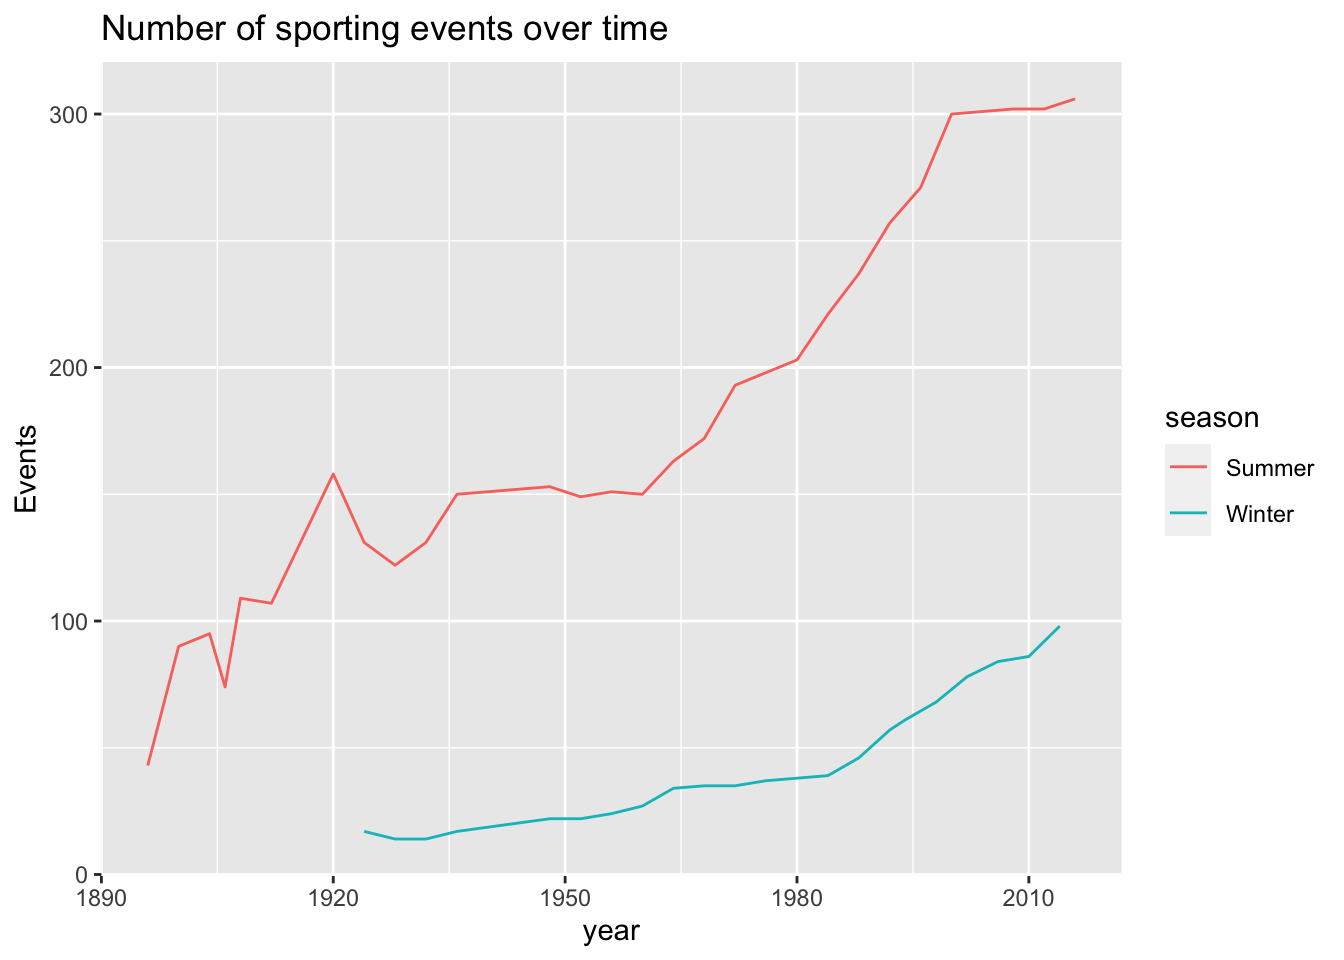
\includegraphics{presentation_files/figure-beamer/unnamed-chunk-9-1.pdf}
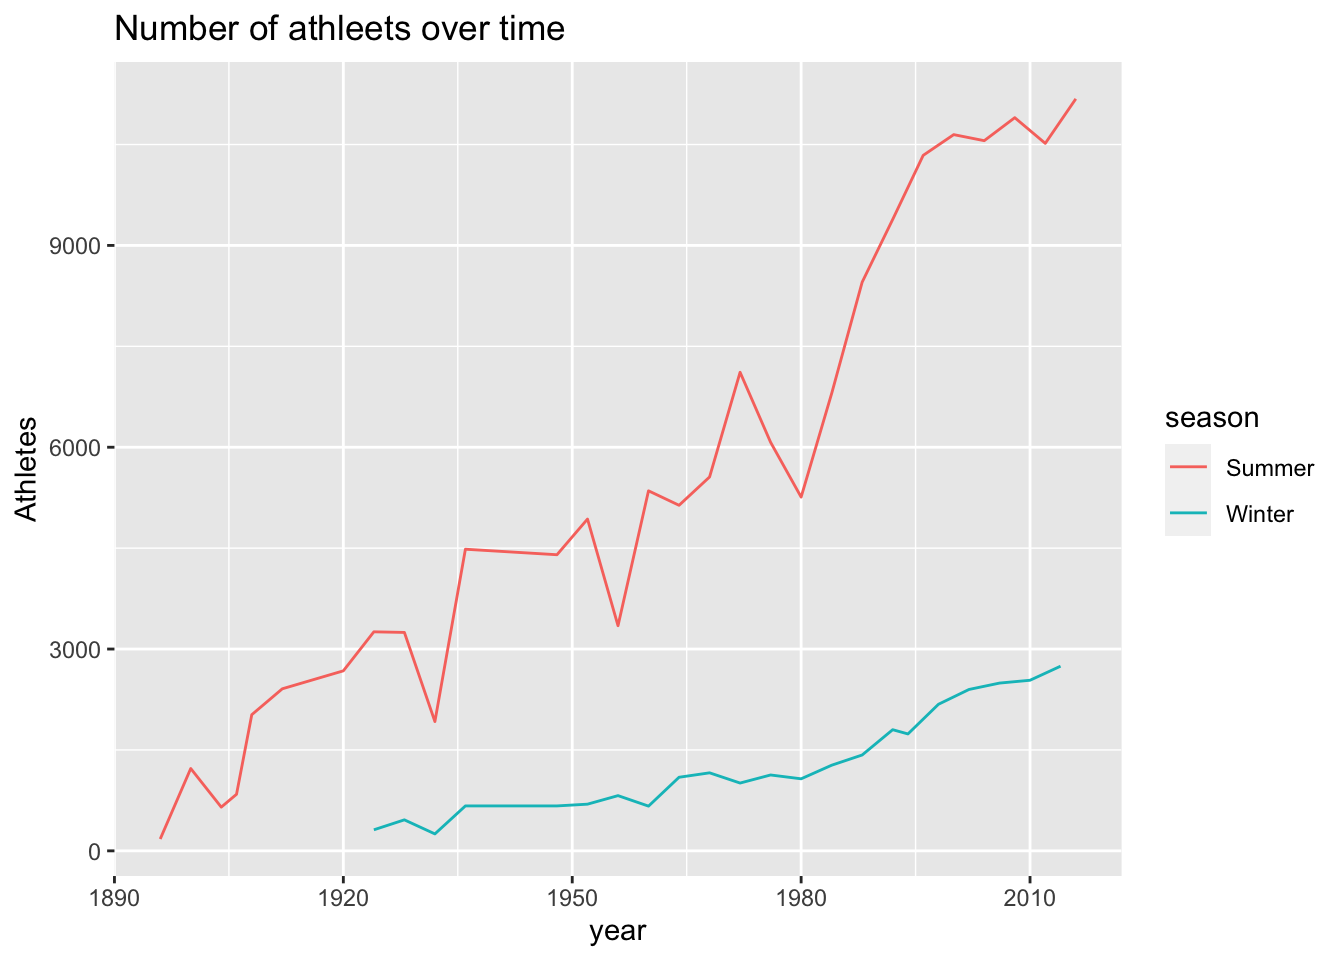
\includegraphics{presentation_files/figure-beamer/unnamed-chunk-9-2.pdf}
\end{block}

\begin{block}{Q3: What is the total number of medals won by each
country?}
\protect\hypertarget{q3-what-is-the-total-number-of-medals-won-by-each-country}{}
\begin{verbatim}
## `summarise()` has grouped output by 'noc'. You can override using the `.groups`
## argument.
\end{verbatim}

\begin{verbatim}
## # A tibble: 362 x 3
## # Groups:   noc [149]
##    noc   medal  Total
##    <fct> <fct>  <int>
##  1 AFG   Bronze     2
##  2 AHO   Silver     1
##  3 ALG   Bronze     8
##  4 ALG   Gold       5
##  5 ALG   Silver     4
##  6 ANZ   Bronze     5
##  7 ANZ   Gold      20
##  8 ANZ   Silver     4
##  9 ARG   Bronze    91
## 10 ARG   Gold      91
## # ... with 352 more rows
\end{verbatim}

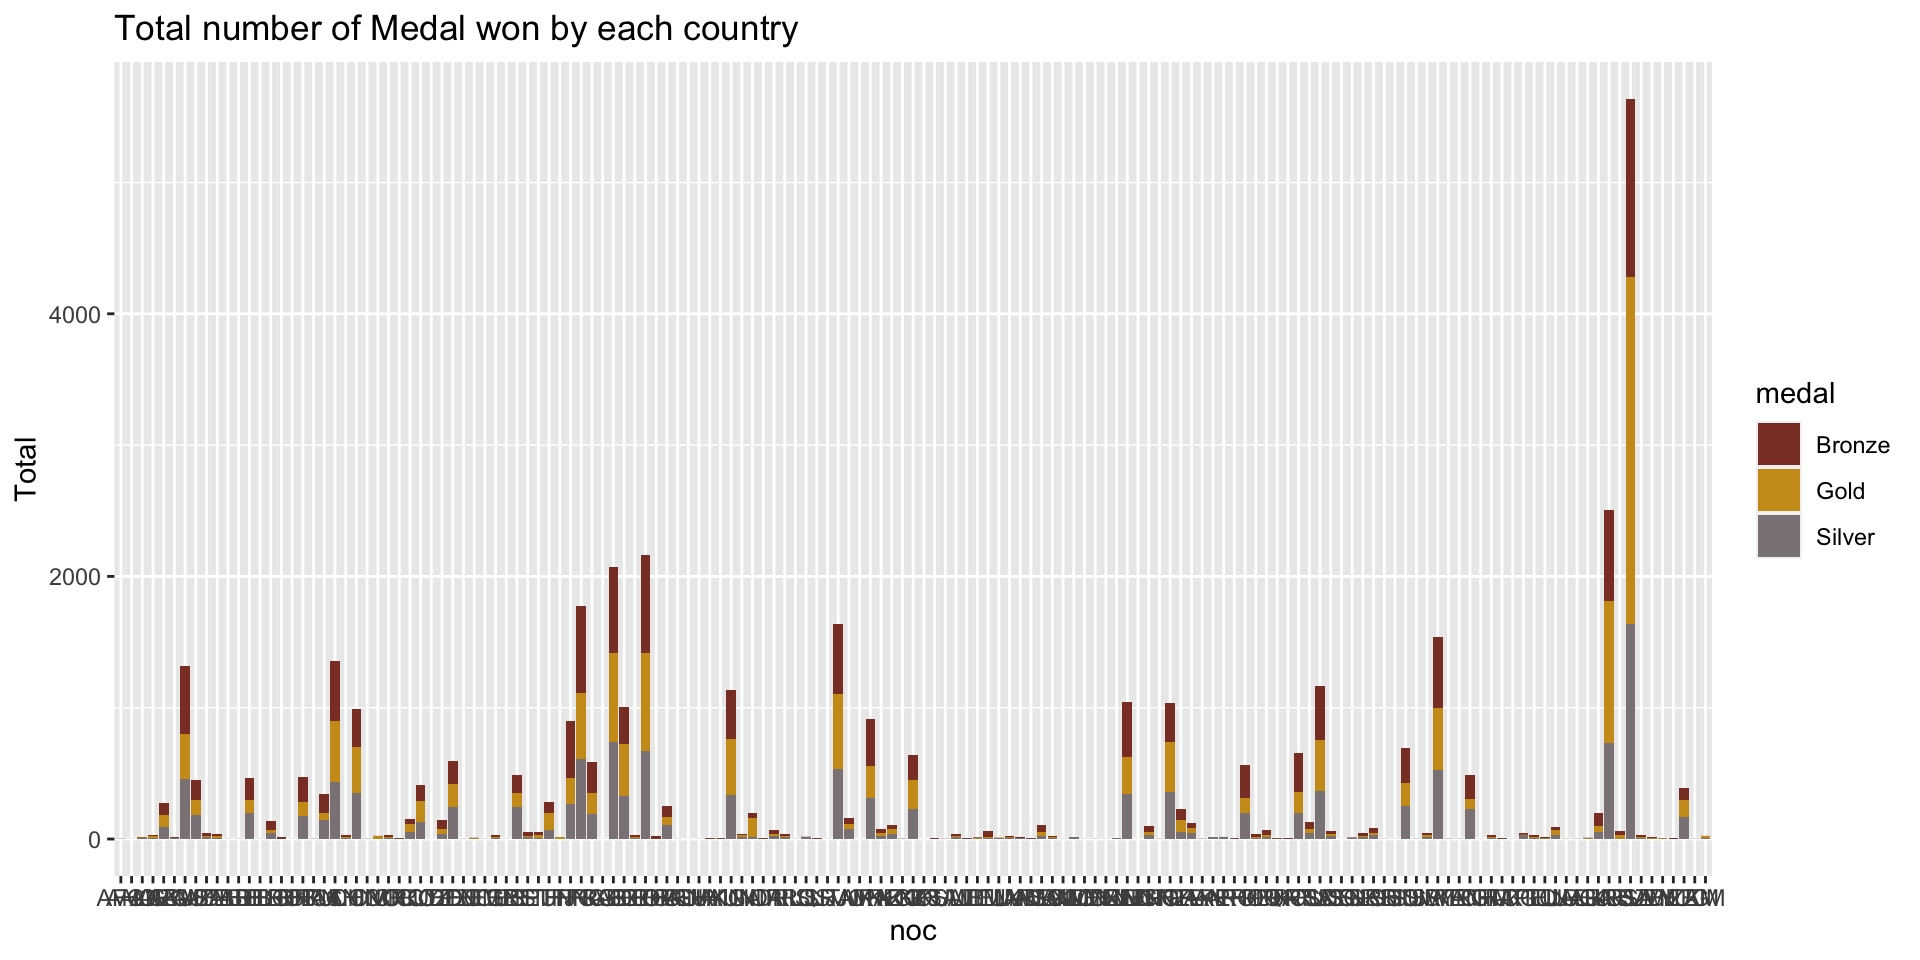
\includegraphics{presentation_files/figure-beamer/unnamed-chunk-10-1.pdf}

\begin{verbatim}
## # A tibble: 498 x 2
##    team                         Total
##    <chr>                        <int>
##  1 A North American Team            4
##  2 Afghanistan                      2
##  3 Algeria                         17
##  4 Ali-Baba II                      5
##  5 Amateur Athletic Association     5
##  6 Amstel Amsterdam                 4
##  7 Ancora                           4
##  8 Angelita                        12
##  9 Antwerpia V                      5
## 10 Aphrodite                        3
## # ... with 488 more rows
\end{verbatim}
\end{block}

\begin{block}{Q4: Who are the top 3 countries that have the most number
of participants over the years and how do we compare them over the
years?}
\protect\hypertarget{q4-who-are-the-top-3-countries-that-have-the-most-number-of-participants-over-the-years-and-how-do-we-compare-them-over-the-years}{}
\begin{verbatim}
## 
##   USA   FRA   GBR   ITA   GER 
## 18853 12758 12256 10715  9830
\end{verbatim}

\begin{block}{United States:}
\protect\hypertarget{united-states}{}
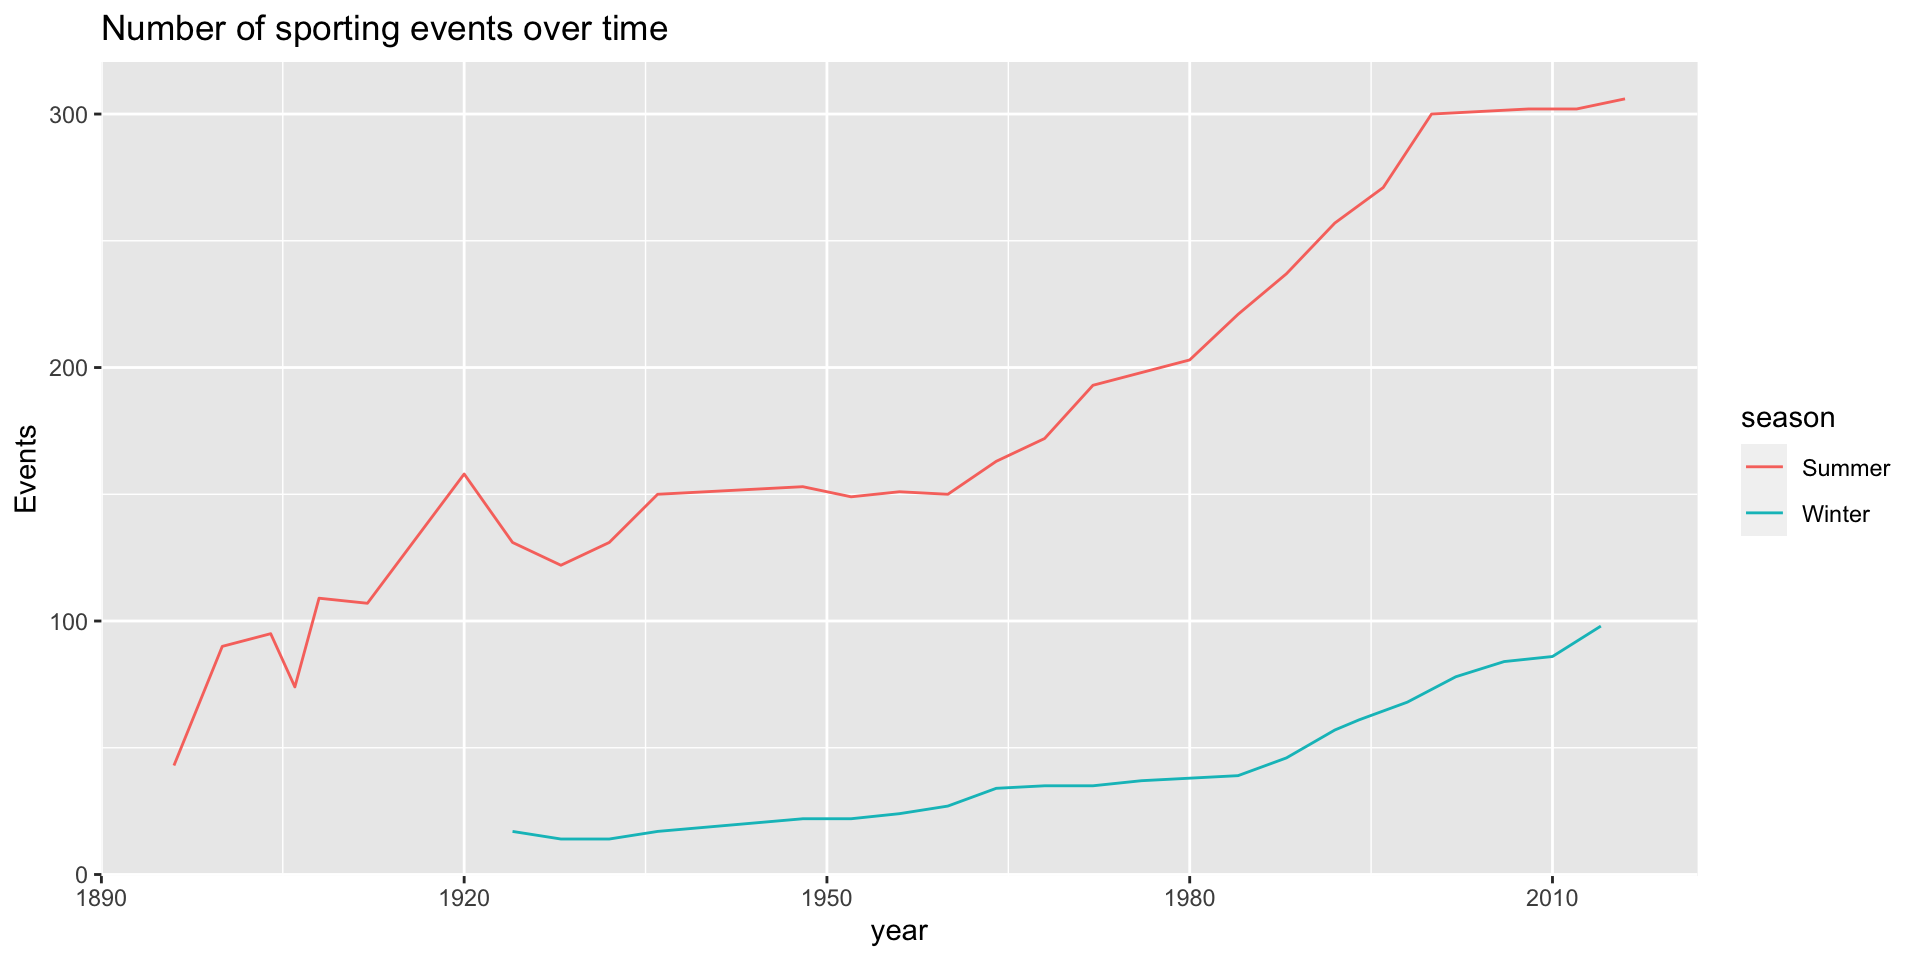
\includegraphics{presentation_files/figure-beamer/unnamed-chunk-12-1.pdf}
\end{block}

\begin{block}{France}
\protect\hypertarget{france}{}
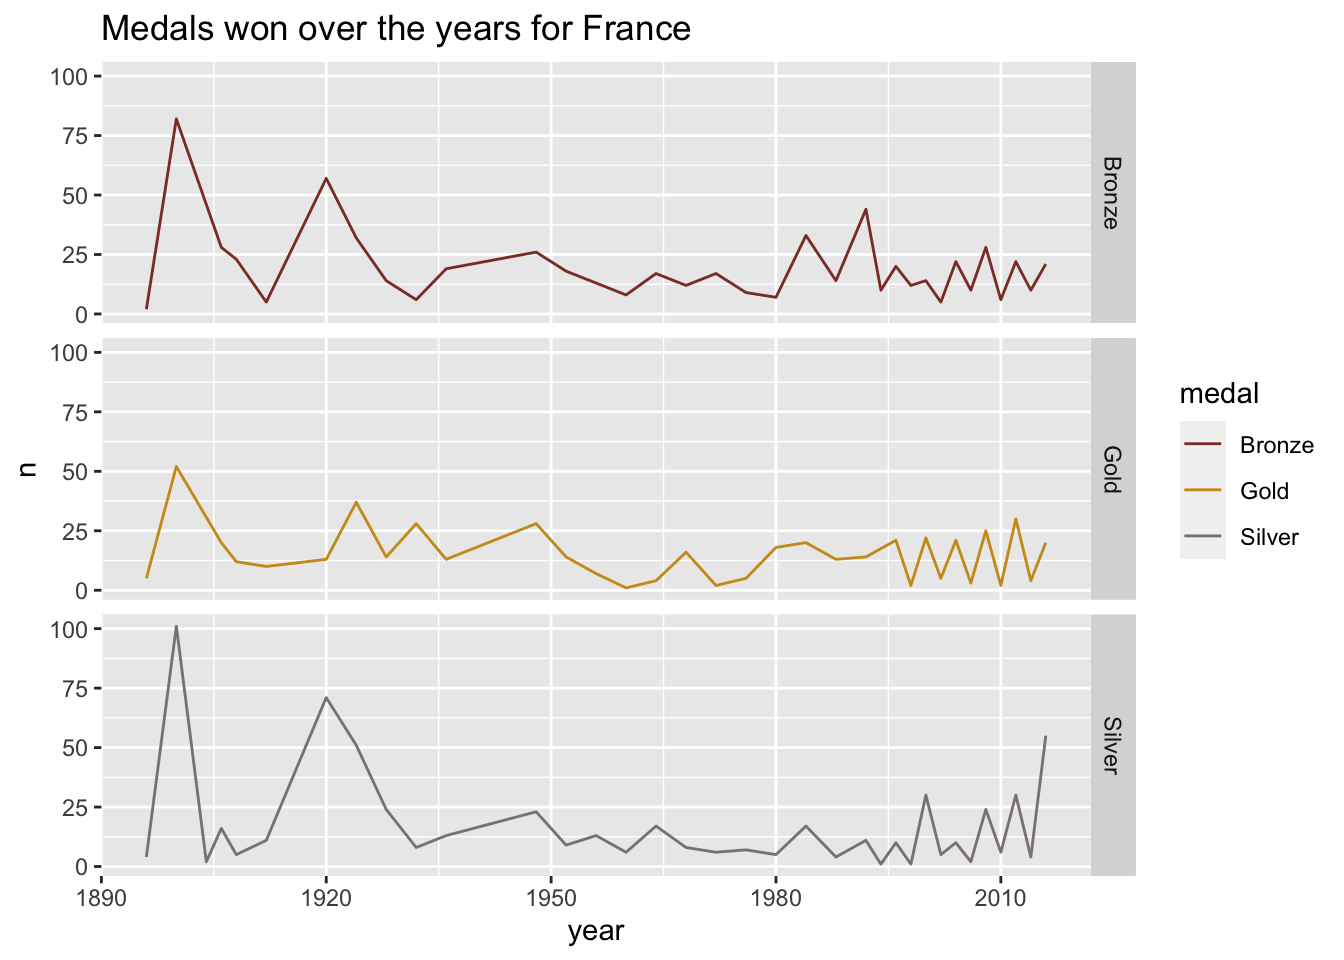
\includegraphics{presentation_files/figure-beamer/unnamed-chunk-13-1.pdf}
\end{block}

\begin{block}{United Kingdom:}
\protect\hypertarget{united-kingdom}{}
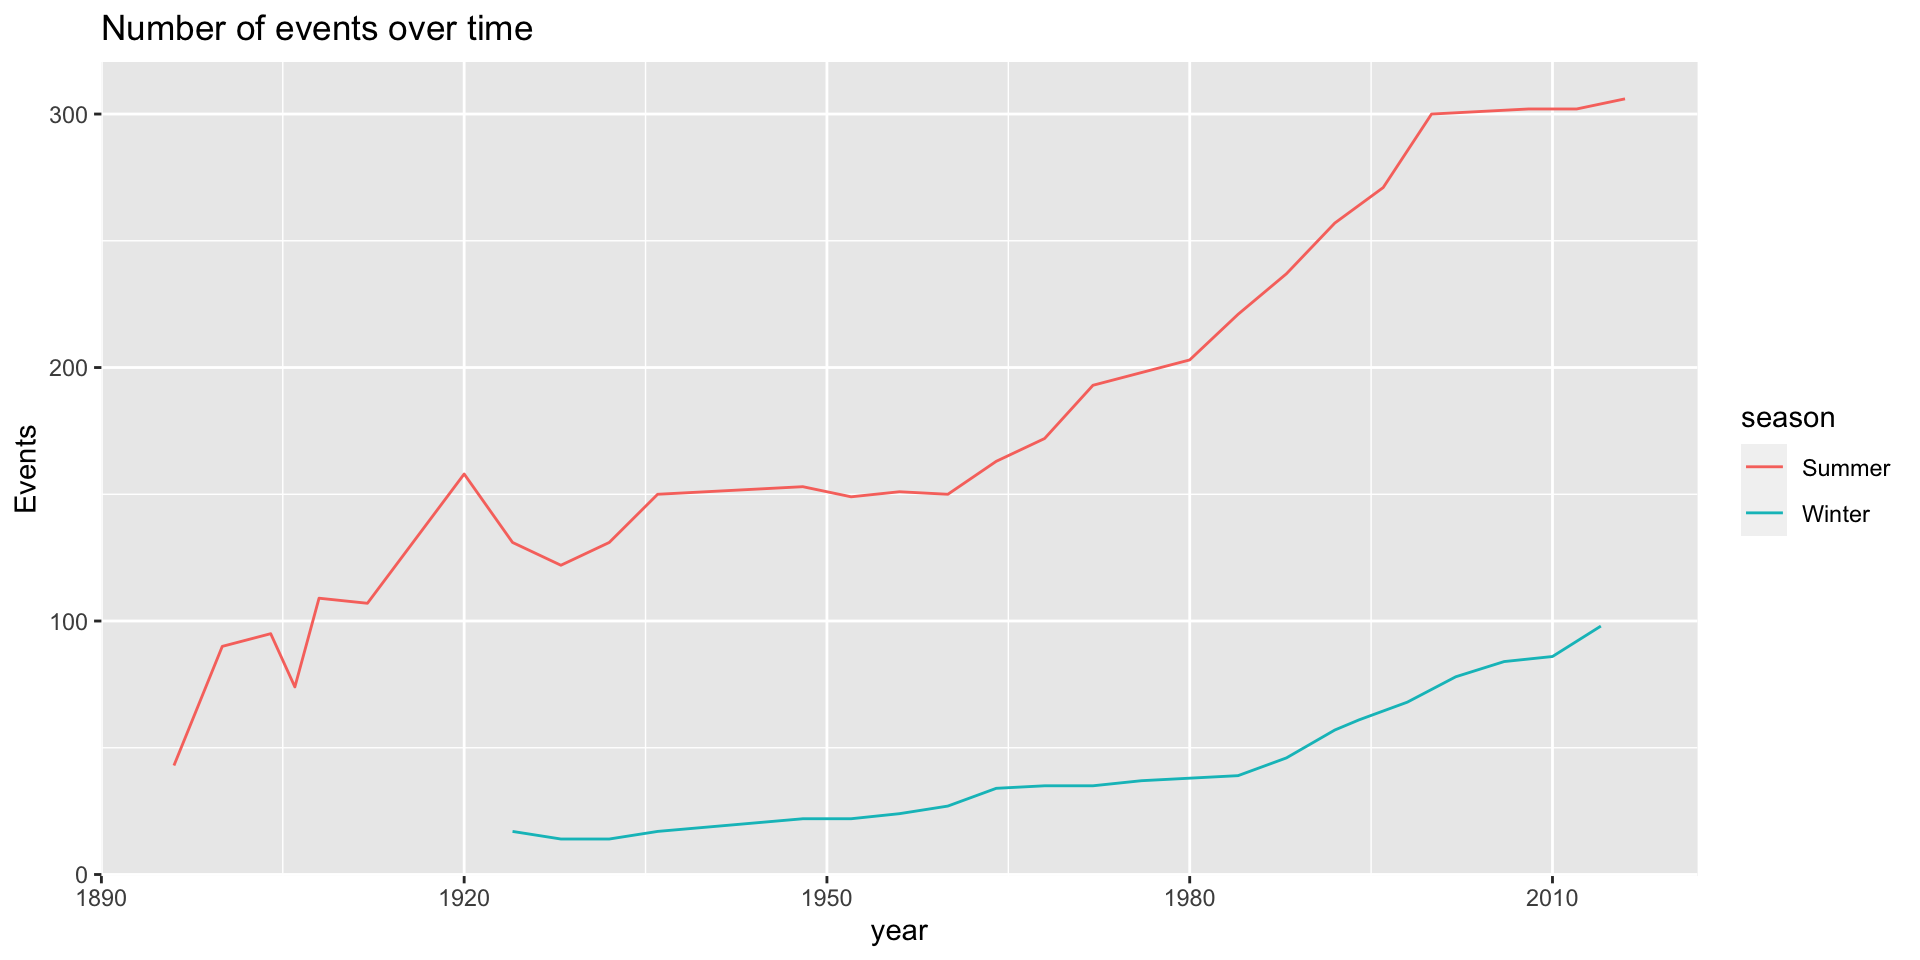
\includegraphics{presentation_files/figure-beamer/unnamed-chunk-14-1.pdf}
\end{block}
\end{block}

\begin{block}{Q5: What is the percentage of the distribution of male and
female athletes throughout the years of Olympic history?}
\protect\hypertarget{q5-what-is-the-percentage-of-the-distribution-of-male-and-female-athletes-throughout-the-years-of-olympic-history}{}
\begin{verbatim}
## `summarise()` has grouped output by 'year'. You can override using the
## `.groups` argument.
\end{verbatim}

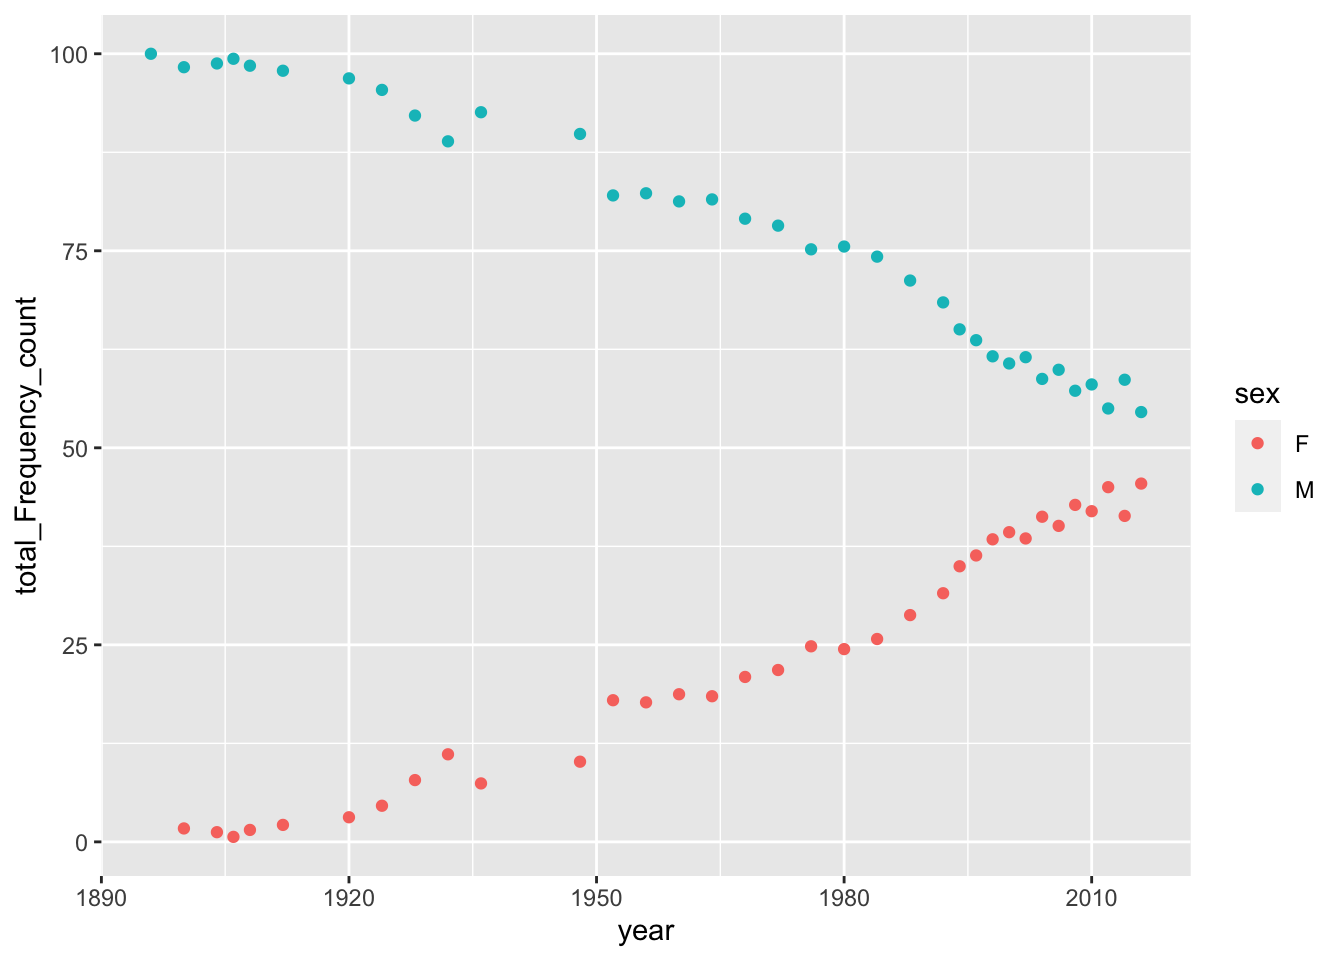
\includegraphics{presentation_files/figure-beamer/unnamed-chunk-15-1.pdf}
\end{block}

\begin{block}{Q6: How many male and females participated in the
Olympics?}
\protect\hypertarget{q6-how-many-male-and-females-participated-in-the-olympics}{}
\begin{verbatim}
## # A tibble: 2 x 2
##   sex    count
##   <fct>  <int>
## 1 F      33981
## 2 M     101590
\end{verbatim}

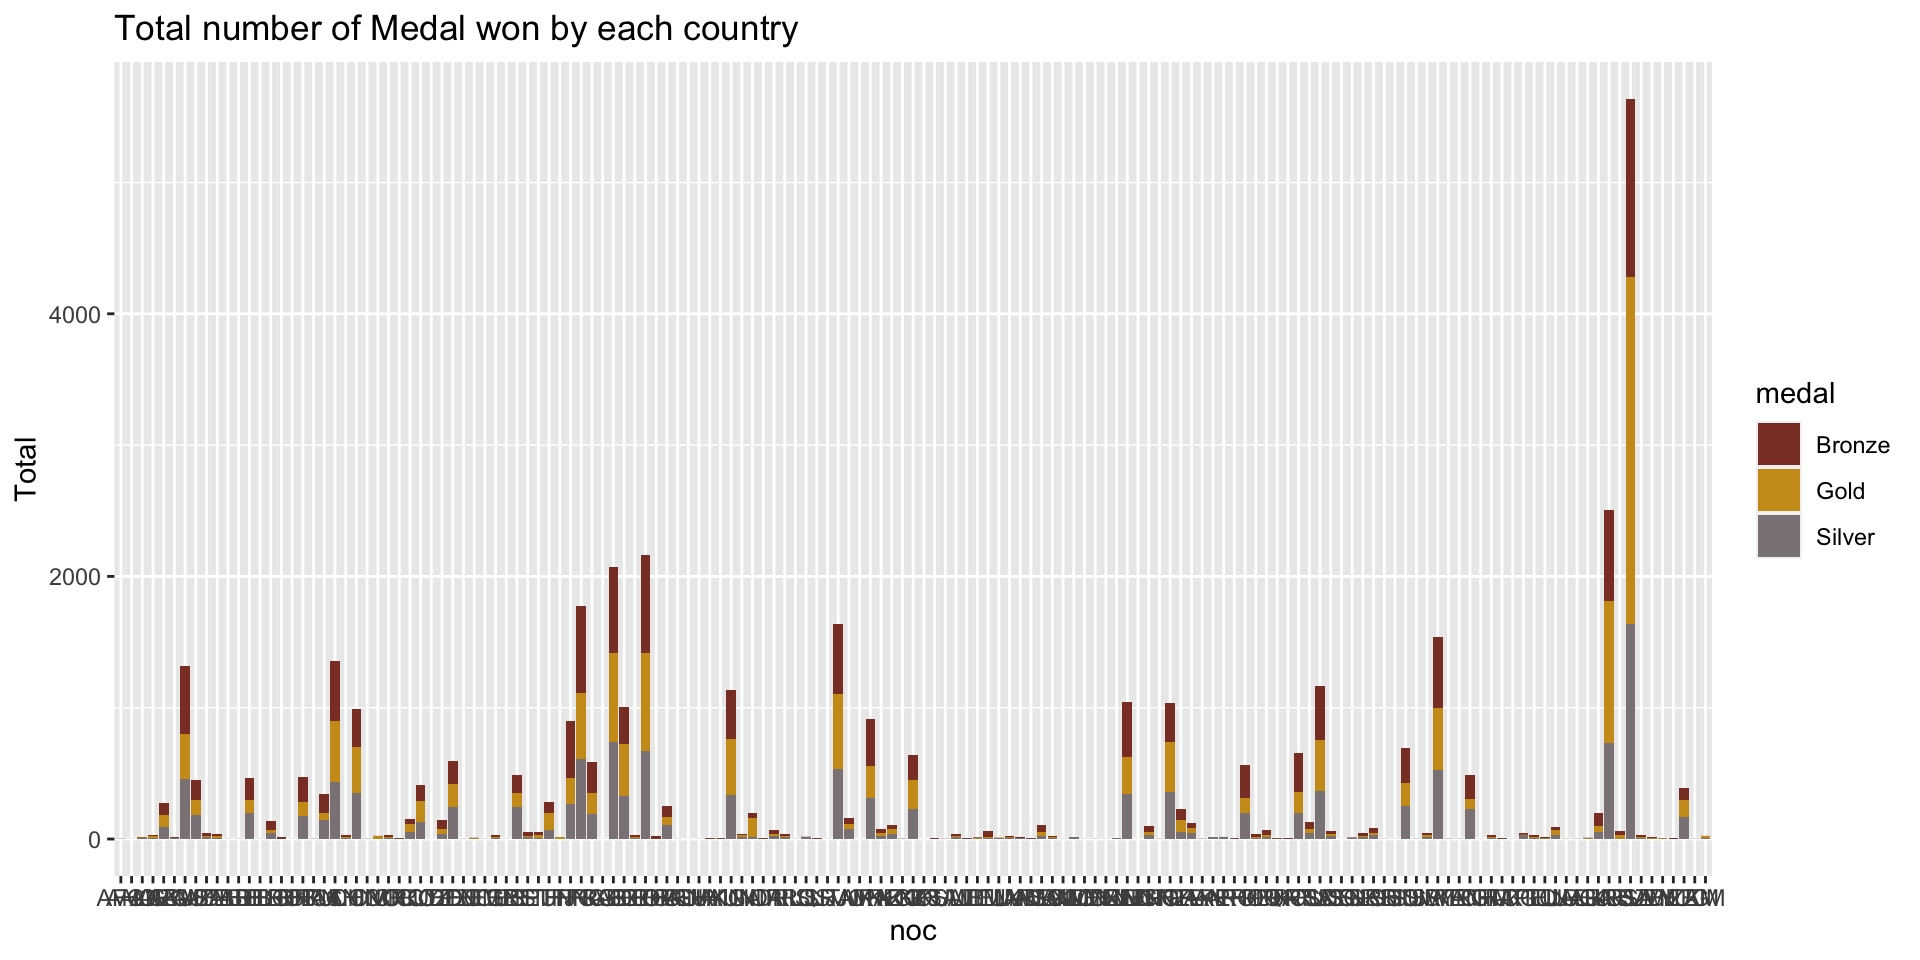
\includegraphics{presentation_files/figure-beamer/unnamed-chunk-16-1.pdf}
\end{block}

\begin{block}{Q7: Can we comparing men and women winners over the years
for summer and winter?}
\protect\hypertarget{q7-can-we-comparing-men-and-women-winners-over-the-years-for-summer-and-winter}{}
\begin{block}{Summer:}
\protect\hypertarget{summer}{}
\begin{verbatim}
## `summarise()` has grouped output by 'year', 'sex', 'medal'. You can override
## using the `.groups` argument.
\end{verbatim}

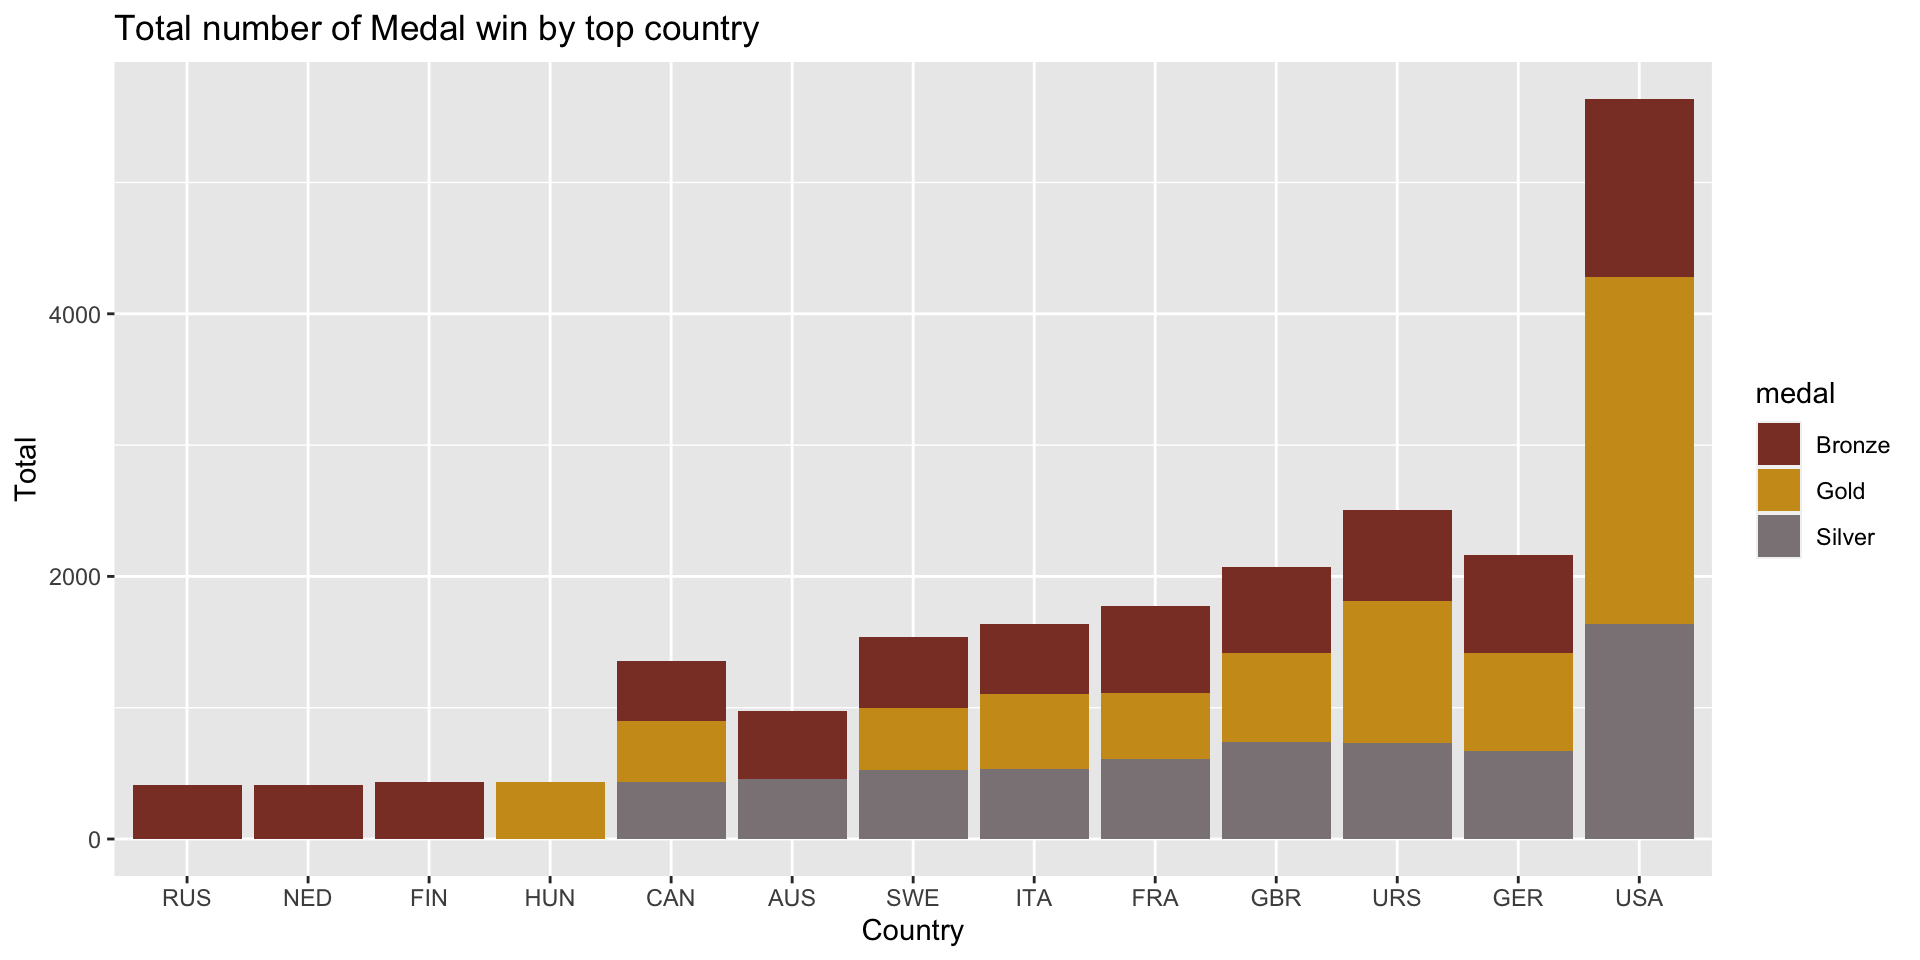
\includegraphics{presentation_files/figure-beamer/unnamed-chunk-17-1.pdf}
\end{block}

\begin{block}{Winter:}
\protect\hypertarget{winter}{}
\begin{verbatim}
## `summarise()` has grouped output by 'year', 'sex', 'medal'. You can override
## using the `.groups` argument.
\end{verbatim}

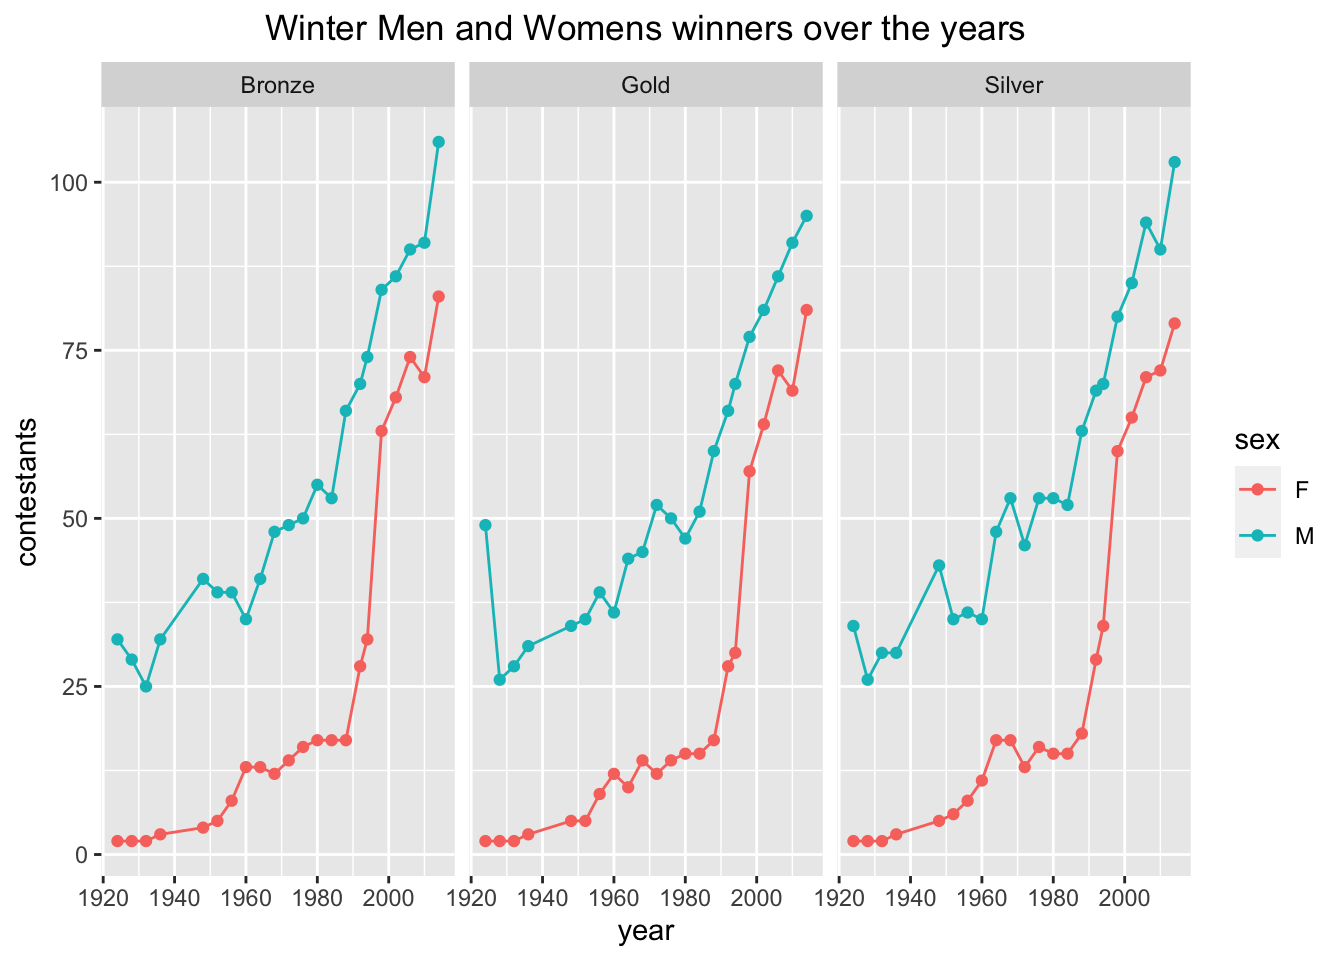
\includegraphics{presentation_files/figure-beamer/unnamed-chunk-18-1.pdf}
\end{block}
\end{block}

\begin{block}{Q8: How many medal have been won by male and female?}
\protect\hypertarget{q8-how-many-medal-have-been-won-by-male-and-female}{}
\begin{verbatim}
## # A tibble: 8 x 3
## # Groups:   sex, medal [8]
##   sex   medal        n
##   <fct> <fct>    <int>
## 1 F     Bronze    3771
## 2 F     Gold      3747
## 3 F     Not win  63269
## 4 F     Silver    3735
## 5 M     Bronze    9524
## 6 M     Gold      9625
## 7 M     Not win 168064
## 8 M     Silver    9381
\end{verbatim}

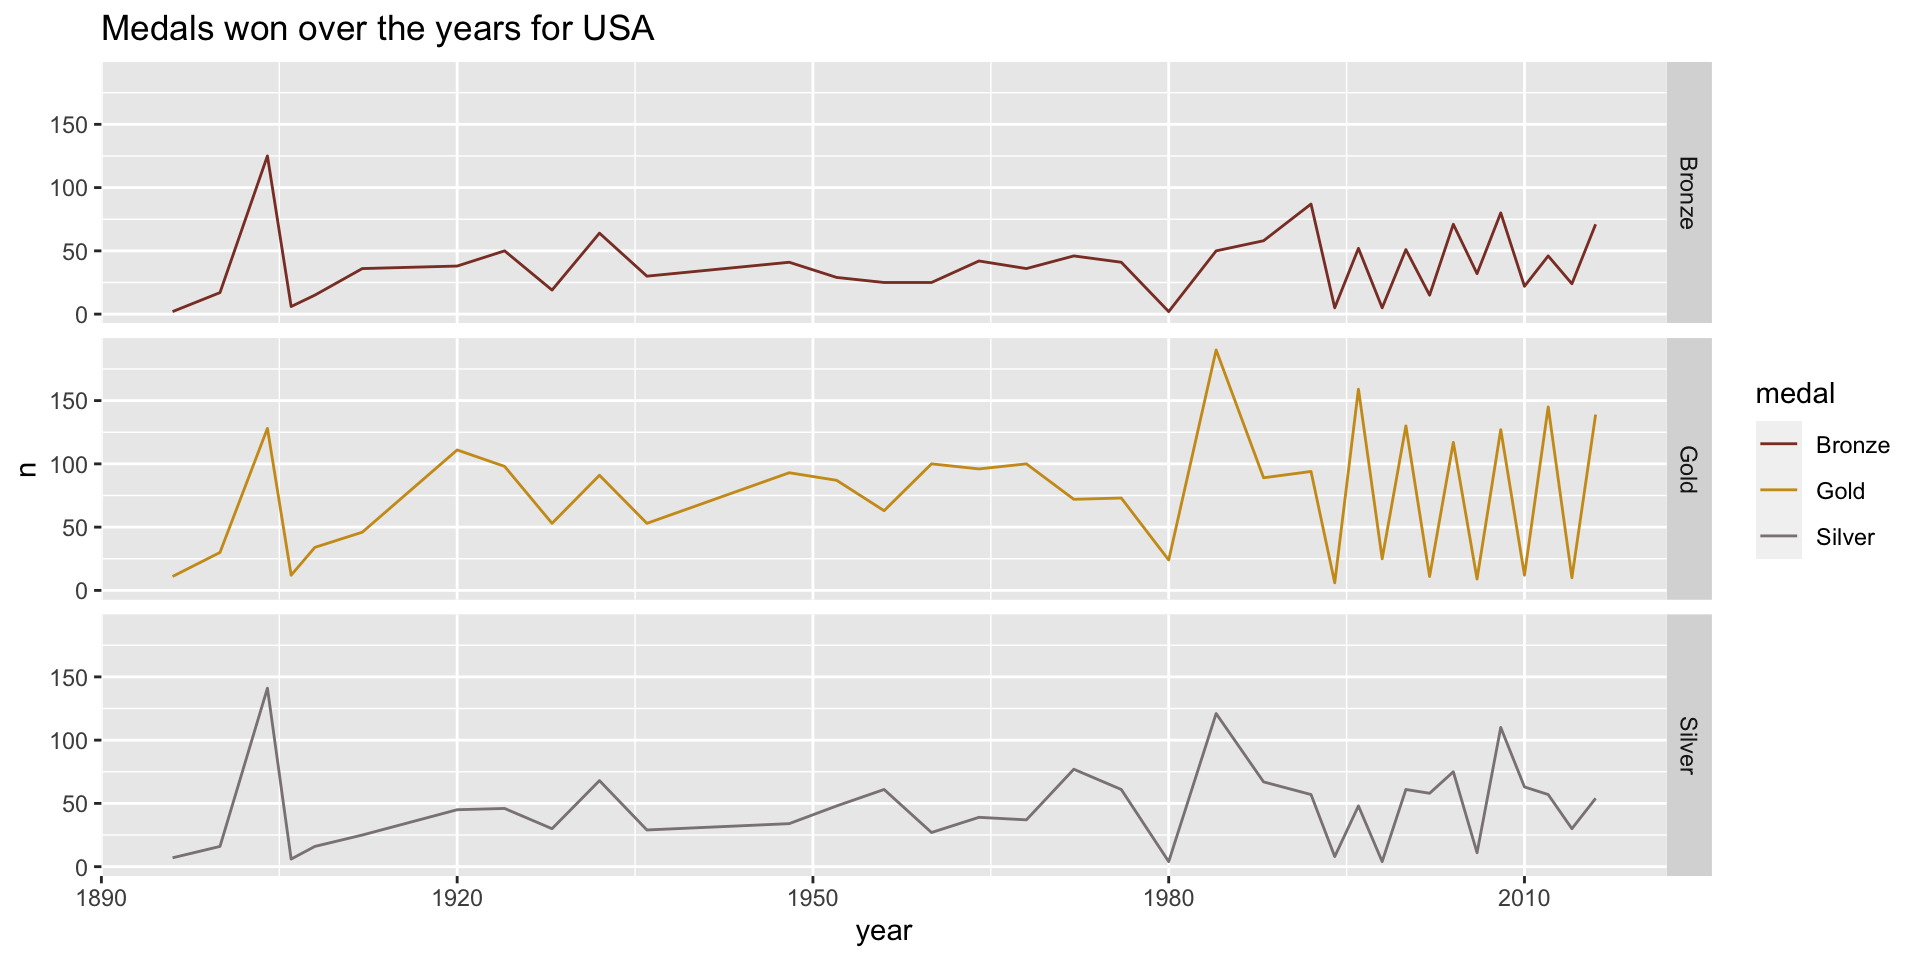
\includegraphics{presentation_files/figure-beamer/unnamed-chunk-19-1.pdf}
\end{block}

\begin{block}{Q9: What is the most productive age for both male and
female athletes in all sorts of sports?}
\protect\hypertarget{q9-what-is-the-most-productive-age-for-both-male-and-female-athletes-in-all-sorts-of-sports}{}
\begin{verbatim}
## `summarise()` has grouped output by 'age'. You can override using the `.groups`
## argument.
\end{verbatim}

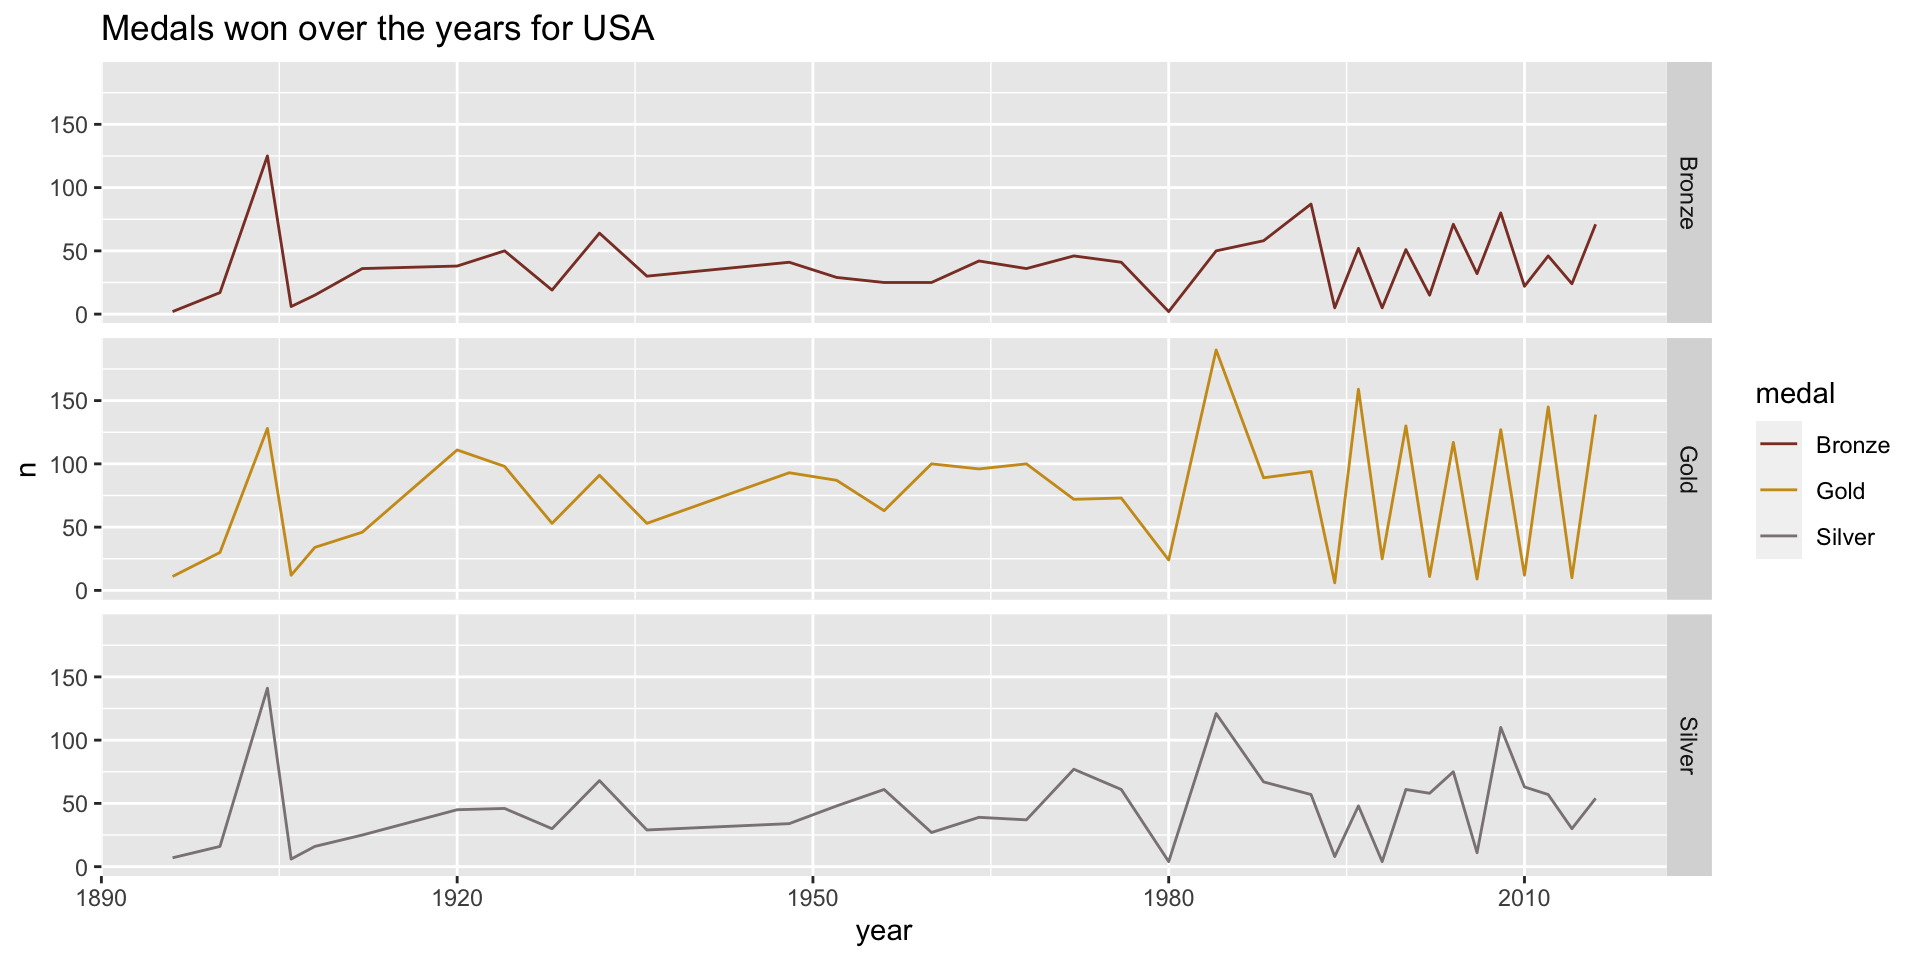
\includegraphics{presentation_files/figure-beamer/unnamed-chunk-20-1.pdf}
\end{block}

\begin{block}{Q10: Is there a relation between athletes' gender and
their winning to their olympic game?}
\protect\hypertarget{q10-is-there-a-relation-between-athletes-gender-and-their-winning-to-their-olympic-game}{}
\begin{verbatim}
## `summarise()` has grouped output by 'sex'. You can override using the `.groups`
## argument.
## `summarise()` has grouped output by 'sex', 'event'. You can override using the
## `.groups` argument.
## `summarise()` has grouped output by 'sex', 'event'. You can override using the
## `.groups` argument.
\end{verbatim}

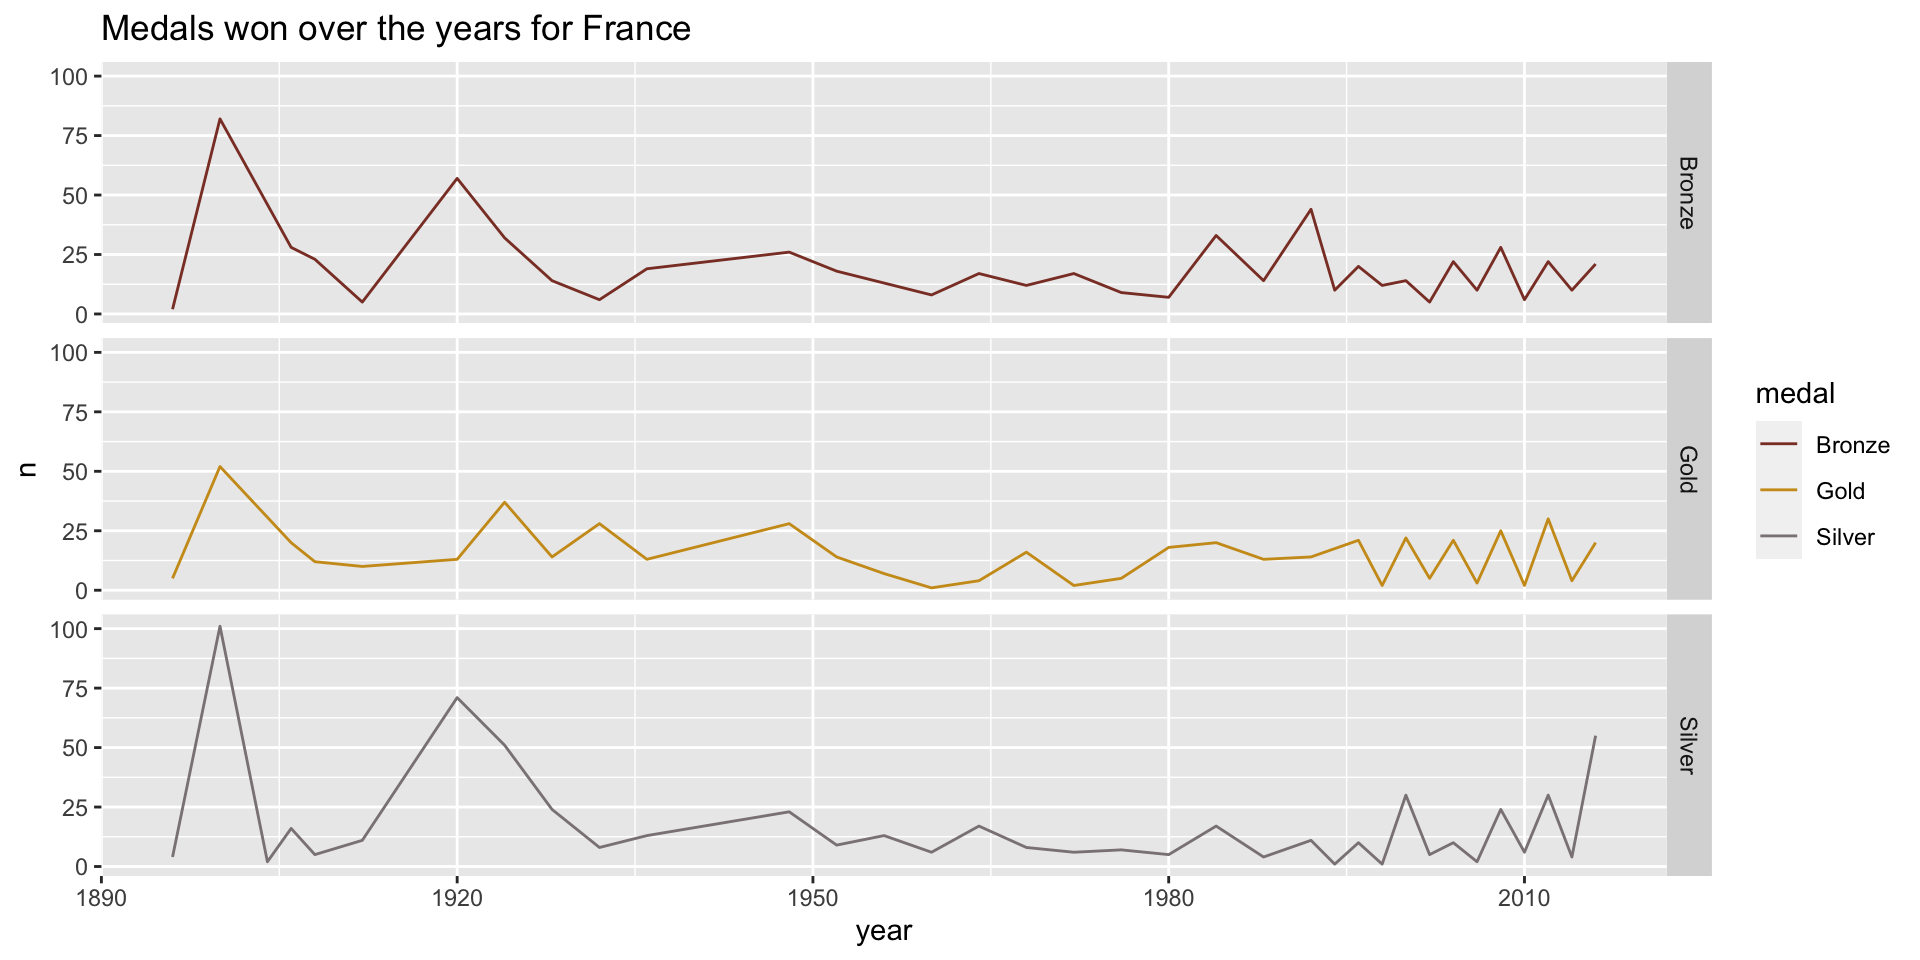
\includegraphics{presentation_files/figure-beamer/unnamed-chunk-21-1.pdf}
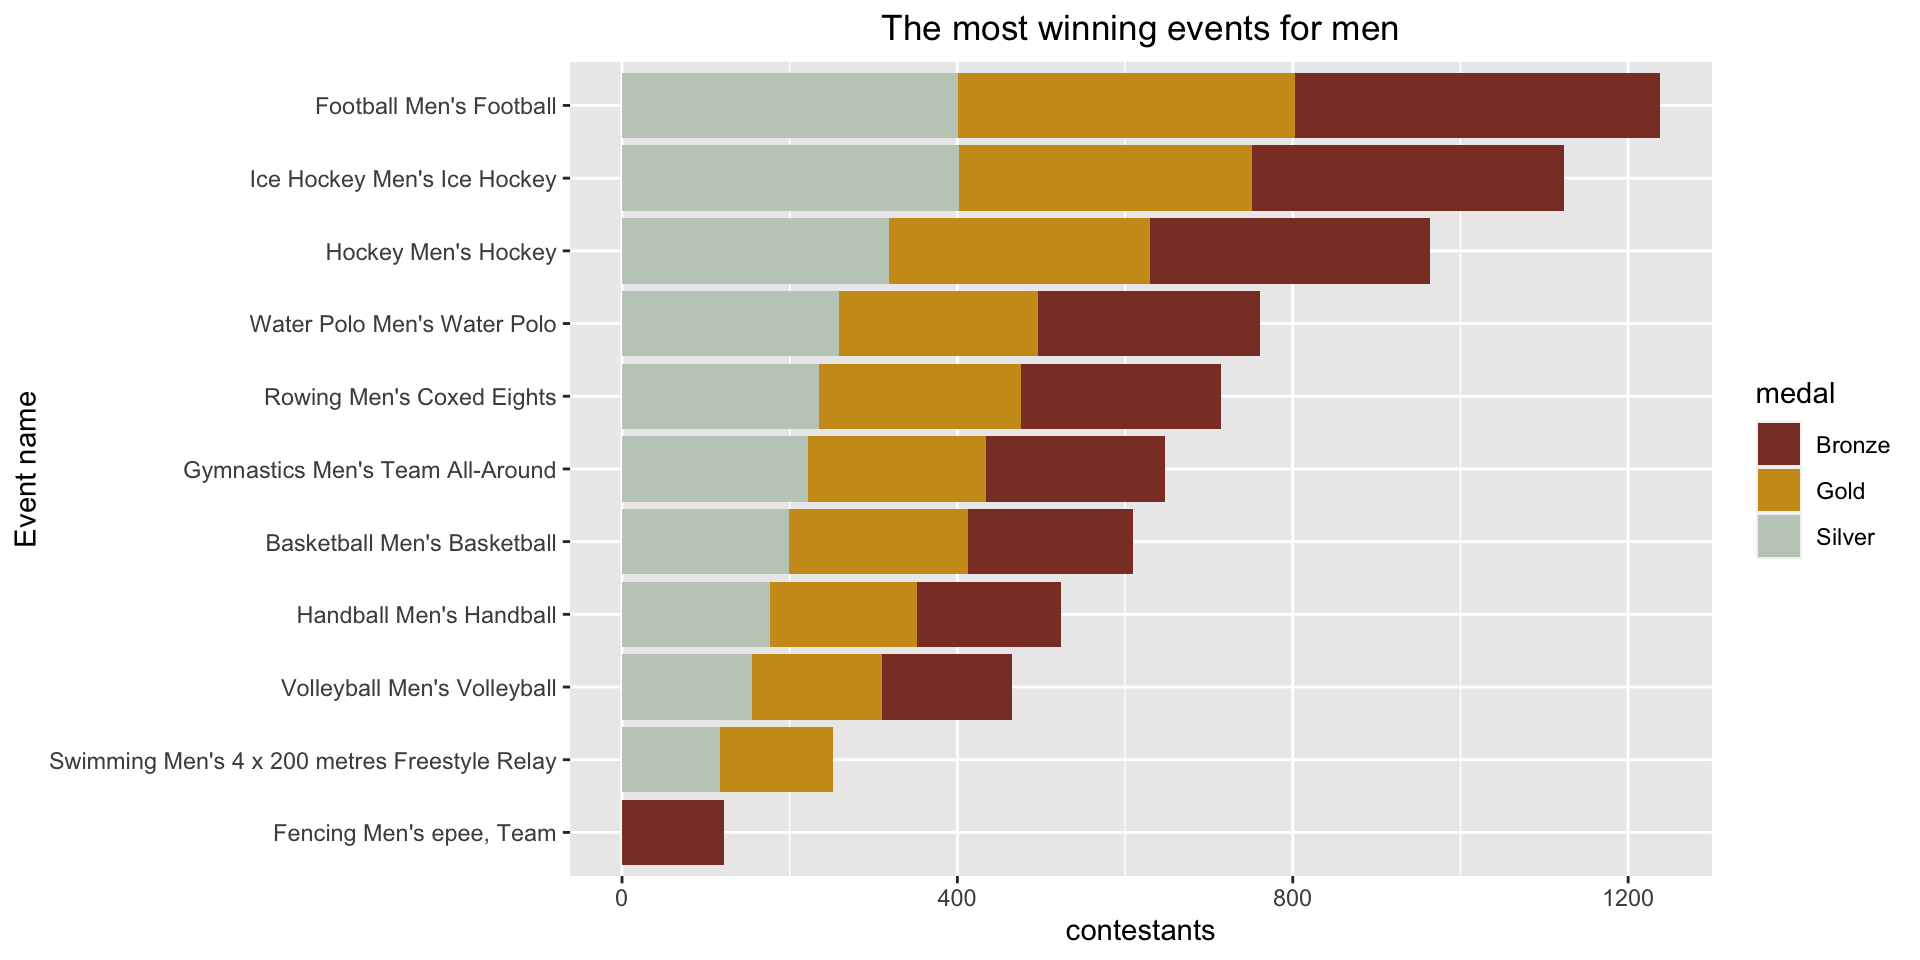
\includegraphics{presentation_files/figure-beamer/unnamed-chunk-21-2.pdf}
\end{block}
\end{frame}

\begin{frame}[fragile]{Step 4 (Hypothesis testing questions):}
\protect\hypertarget{step-4-hypothesis-testing-questions}{}
\begin{block}{Women growth since they joined the olympics}
\protect\hypertarget{women-growth-since-they-joined-the-olympics}{}
\begin{verbatim}
## `summarise()` has grouped output by 'year', 'sex'. You can override using the
## `.groups` argument.
\end{verbatim}

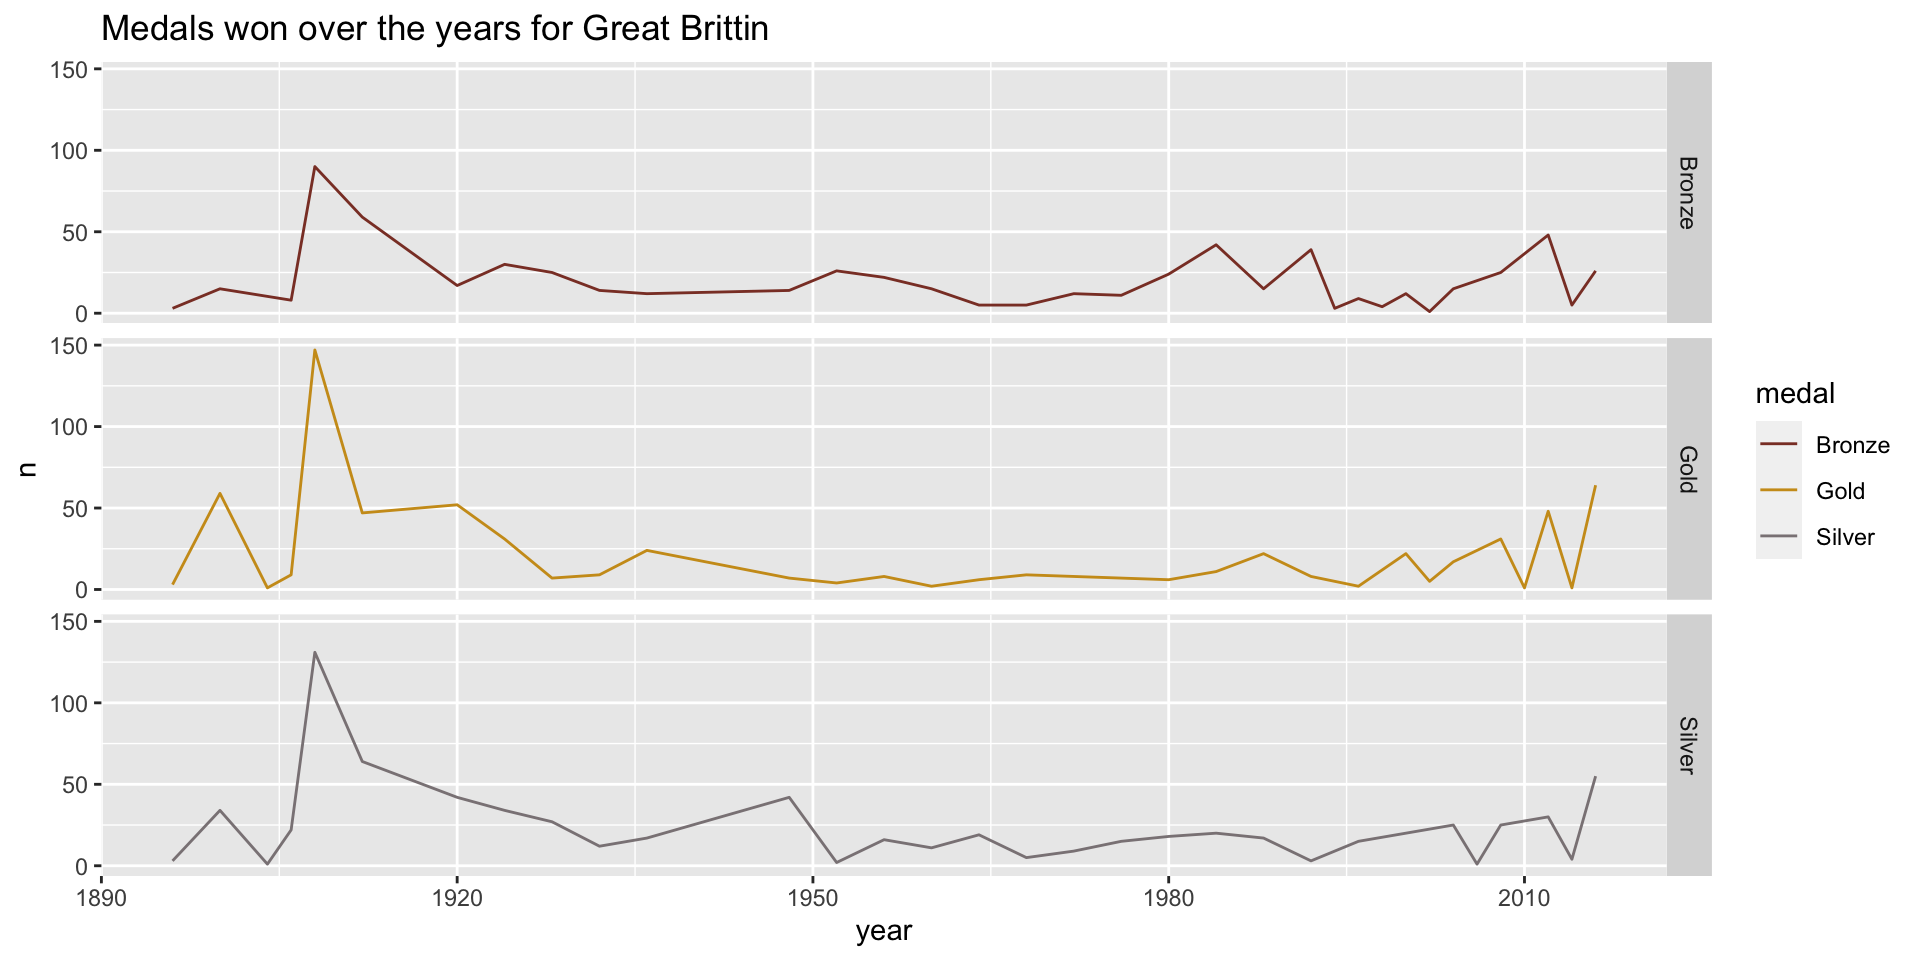
\includegraphics{presentation_files/figure-beamer/unnamed-chunk-22-1.pdf}
\end{block}

\begin{block}{Men growth vs.~women growth}
\protect\hypertarget{men-growth-vs.-women-growth}{}
\begin{verbatim}
## `summarise()` has grouped output by 'year', 'sex'. You can override using the
## `.groups` argument.
\end{verbatim}

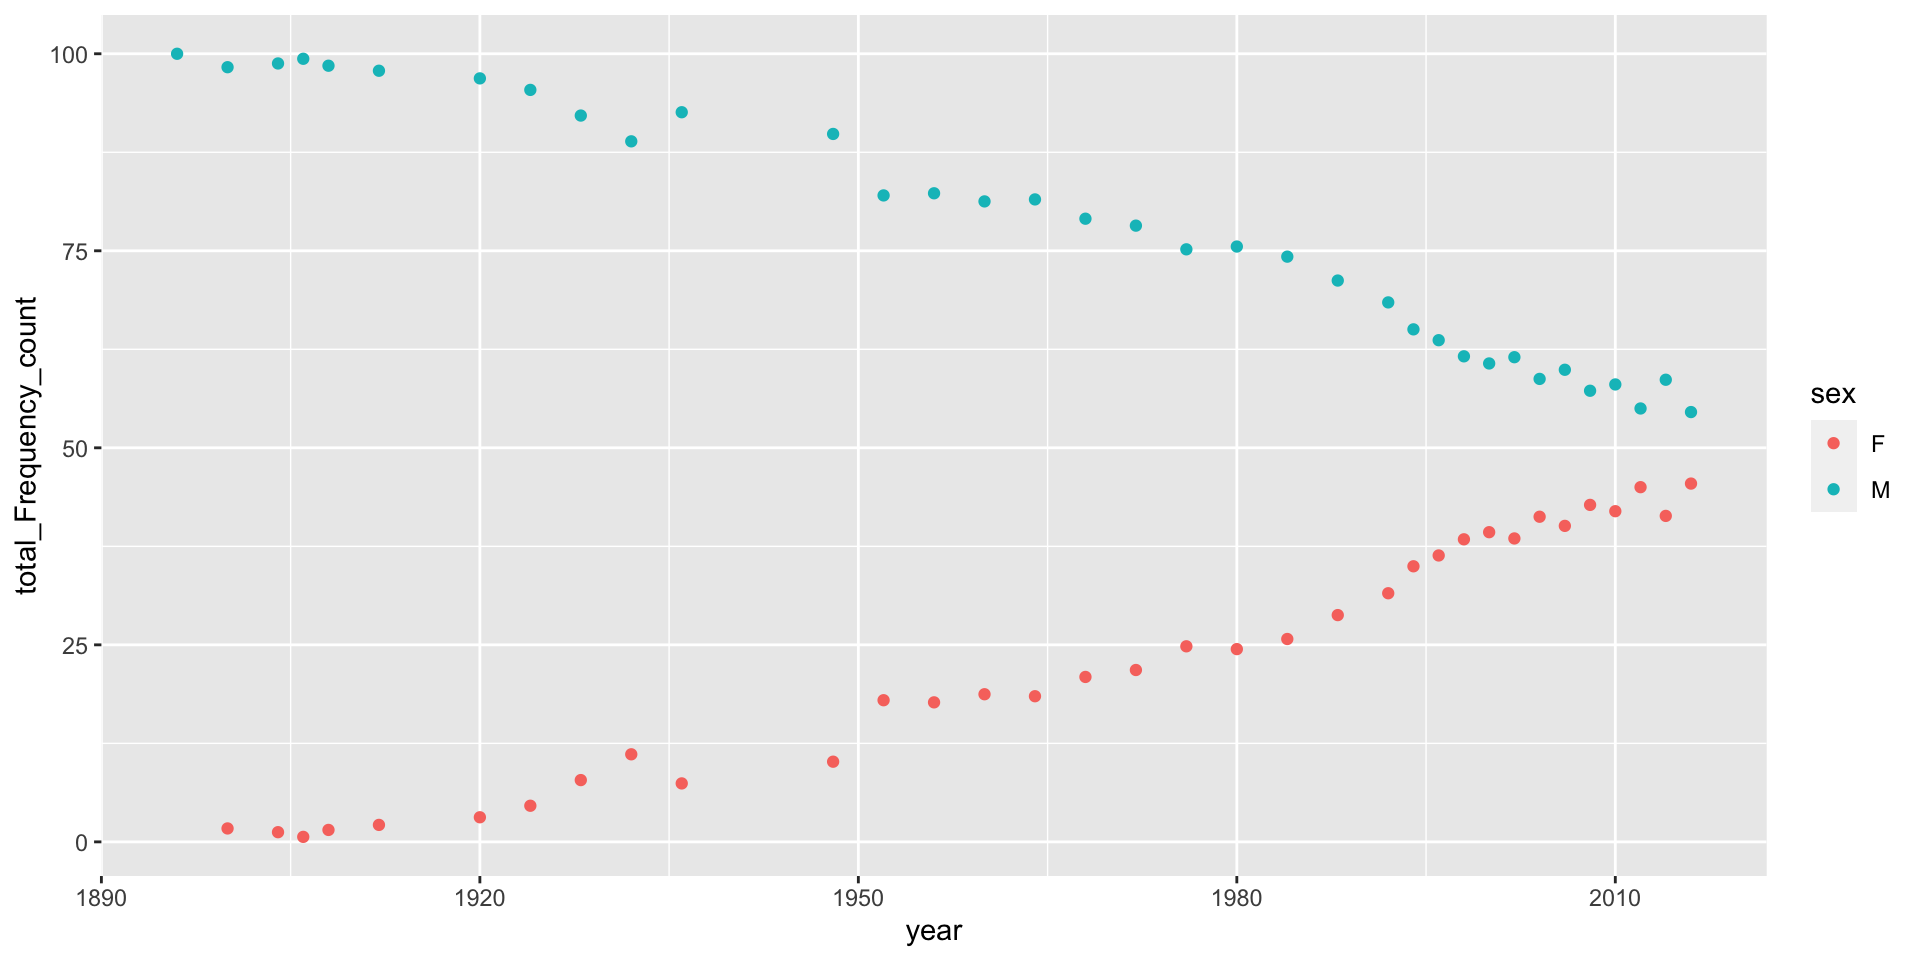
\includegraphics{presentation_files/figure-beamer/unnamed-chunk-23-1.pdf}
\end{block}
\end{frame}

\begin{frame}{Step 5 (Summary):}
\protect\hypertarget{step-5-summary}{}
\end{frame}

\end{document}
